\documentclass[dosguias]{tesis-postgrado}
% Opciones: dosguias, propuesta

\begin{document}
\baselineskip 23pt
\frontmatter								% Utiliza numeración romana

% ### Cubierta de la tesis ###
\thispagestyle{empty}
\facultad{Ingeniería}
\departamento{Ingeniería Informática}
\grado{Magíster en Ingeniería Informática}

\titulo{T\'itulo de la tesis}

\autor{Miguel \'Angel C\'arcamo V\'asquez}
\email{miguel.carcamo@usach.cl}
\run{18.294.093-3}		% S\'olo necesario en propuesta
\telefono{22222222}		% S\'olo necesario en propuesta
\annoingreso{2010}

\fecha{Mi\'ercoles}{12}{Diciembre}{2016}

\profesorguia{Fernando Rannou Fuentes}
\profesorcoguia{Pablo E. Román}


\ciudad{Santiago}
\pais{Chile}

\makecubierta


% ### Páginas preliminares de la tesis ###
\pagestyle{fancy}
\renewcommand{\headrulewidth}{0pt}		% Hace que no aparezca la línea horizontal superior al principio de estas páginas
\fancyhead[L]{}
\fancyhead[C]{}
\fancyhead[R]{}

\makecopyright							% Si es propuesta no se mostrará
% ### Dedicatoria y agredecimientos de la tesis ###
\dedicatoria{
Dedicado a...
}
		% En caso de no querer agregarlos, comente esta línea
\begin{agradecimiento}
Agradezco a
\end{agradecimiento}

\pagestyle{fancy}

% ### Índices ###
\tableofcontents							%% Tabla de contenido

\listoftables							%% Indice de tablas
\addcontentsline{toc}{chapter}{Índice de tablas} % Comando para agregar el índice a la Tabla de Contenido

\listoffigures							%% Indice de figuras
\addcontentsline{toc}{chapter}{Índice de ilustraciones} % Comando para agregar el índice a la Tabla de Contenido

\listofalgorithms						%% Indice de algoritmos
\addcontentsline{toc}{chapter}{Índice de algoritmos} % Comando para agregar el índice a la Tabla de Contenido

\resumenCastellano{
Lorem ipsum dolor sit cuchufl\'i barquillo bac\'an jote gamba listeilor po cahu\'in, luca mel\'on con vino pichanga coscacho ni ah\'i peinar la muñeca chuchada al chancho achoclonar. Chorrocientos pituto ubicatex huevo duro bolsero cachureo el hoyo del queque en cana huev\'on el año del loly hacerla corta impeque de miedo quilterry la raja longi ñecla. Hilo curado rayuela carrete quina guagua lorea piola ni ah\'i.

\vspace*{0.5cm}
\KeywordsES{Palabras; Claves}
}

\newpage

\resumenIngles{
Contrary to popular belief, Lorem Ipsum is not simply random text. It has roots in a piece of classical Latin literature from 45 BC, making it over 2000 years old. Richard McClintock, a Latin professor at Hampden-Sydney College in Virginia, looked up one of the more obscure Latin words, consectetur, from a Lorem Ipsum passage, and going through the cites of the word in classical literature, discovered the undoubtable source. Lorem Ipsum comes from sections 1.10.32 and 1.10.33 of "de Finibus Bonorum et Malorum" (The Extremes of Good and Evil) by Cicero, written in 45 BC. This book is a treatise on the theory of ethics, very popular during the Renaissance. The first line of Lorem Ipsum, "Lorem ipsum dolor sit amet..", comes from a line in section 1.10.32.

The standard chunk of Lorem Ipsum used since the 1500s is reproduced below for those interested. Sections 1.10.32 and 1.10.33 from "de Finibus Bonorum et Malorum" by Cicero are also reproduced in their exact original form, accompanied by English versions from the 1914 translation by H. Rackham.

\vspace*{0.5cm}
\KeywordsEN{Key; words}
}


% ### Cuerpo de la tesis ###
\mainmatter								% Reinicia el contador de páginas para partir de 1 y usando números arábicos.

% ### Configuración del header ###
\pagestyle{fancy}
\renewcommand{\headrulewidth}{0.4pt}		%Hace que vuelva a aparecer la linea horizontal
\fancyhead[LE,RO]{\slshape \leftmark}	%Hace que se muestre el título del capítulo en las páginas que no son la primera de cada capítulo

% ### Capítulos de la tesis ###
\chapter{Introducci\'on}
\label{cap:introduccion}

\section{Antecedentes y motivaci\'on}
\label{intro:motivacion}
El \textit{Atacama Large Millimeter/Submillimiter Array} es un instrumento revolucionario en su concepto científico, su diseño de ingeniería y su organización como un esfuerzo científico global. Construido en el desierto de Atacama de Chile septentrional a una altitud de 5.000 metros sobre el nivel del mar en el llano Chajnantor, ALMA cuenta con 66 antenas de alta precisión funcionando juntas en longitudes de onda milimétricas y submilimétricas. Gracias a su alta resolución y sensibilidad, ALMA abre una “ventana” totalmente nueva al Universo, permitiendo a los científicos desenmarañar misterios astronómicos importantes y de muchos años, explorando nuestros orígenes cósmicos \citep{alma}.

ALMA captura señales del cielo con dos o más antenas combinadas con el fin de analizar  la señal y así obtener información acerca de la fuente que emite dicha señal (ya sea una estrella, planeta, galaxia u otro objeto astronómico). De esta forma, combinando las ondas de radio recolectadas por muchas antenas es posible construir una imagen. Estas imágenes son comparables con un hipotético telescopio gigante o una antena de 14.000 metros de diámetro. Como la construcción y operación de una antena de tal tamaño es técnicamente imposible, lo factible es construir muchas antenas pequeñas y combinar su salida \citep{howalma}.

Sin embargo, este problema no es tan simple como parece, puesto que para la reconstrucción de las imágenes se necesitan algoritmos especializados. Actualmente existen dos grandes tipos de algoritmos: aquellos basados en transformaciones lineales y aquellos con un soporte Bayesiano, no lineal.

Estos últimos tienen una base matemática sólida, pero fueron dejados de lado por su pobre rendimiento computacional. Es por ello que gracias al desarrollo del hardware, especialmente de las GPU, se pretende acelerar estos algoritmos para tener imágenes de mejor calidad en un tiempo menor al que se obtiene con soluciones secuenciales.

\section{Descripci\'on del problema}
\label{intro:problema}

\subsection{Estado del arte}
\label{sec:estadodelarte}


La reconstrucción de imágenes usando radiointerferómetros que captan una señal del cielo a medida que rota la tierra es llamado un problema \textit{ill-posed} \citep{chen}, debido a la irregularidad de los muestreos Nyquist en el dominio de Fourier. Estos muestreos resultan en \textit{aliasing} o sobreposición de ondas en la imagen debido a los altos lóbulos laterales en la respuesta del \textit{array} de antenas. Es importante entender que obtener imágenes de alta calidad depende tanto de contar con los mejores equipos como con las mejores técnicas de reconstrucción. En ese sentido, cada generación de radiotelescopios involucra un esfuerzo en el desarrollo de \textit{hardware}. Sin embargo, para explotar las capacidades de ese \textit{hardware} se requiere una constante mejora en los enfoques de reconstrucción de imágenes para poder igualar la sensibilidad del receptor.

Durante los últimos 40 años, múltiples técnicas de deconvolución han sido desarrolladas para resolver el problema mencionado anteriormente. 

La idea básica detrás de un algoritmo de deconvolución es explotar un conocimiento \textit{a-priori} de la imagen. El primer algoritmo, y la más popular de estas técnicas en el campo de la astronomía, es el método CLEAN propuesto por Högbom \citep{CLEAN}. Este método se basa en aproximar la imagen usando lo que se denomina como \textit{dirty image}. La \textit{dirty image} se muestra en la ecuación \ref{eq:dirtyimage} y es la imagen obtenida luego de aplicar la transformada de Fourier inversa sobre el conjunto de visibilidades $V$ multiplicada por la función de muestreo $S(u,v)$, tal que $S(u,v)=1$ donde exista una visibilidad y $S(u,v)=0$ si no existe. Las coordenadas $(u,v)$ representan las coordenadas de las mediciones en el plano de Fourier esparcidos de forma irregular. Por otra parte los puntos $(x,y)$ representan las coordenadas planas en la imagen escalada. 

\begin{equation}
I^{D}(x,y) = \int\int V(u,v)S(u,v)e^{2\pi i(ux+vy)}\;du\,dv
\label{eq:dirtyimage}
\end{equation}

CLEAN supone que la imagen verdadera ($I^{T}$) puede ser obtenida mediante un muestreo completo en el dominio de Fourier como en la ecuación \ref{eq:fullcoverage}.

\begin{equation}
I^{T}(x,y) = \int\int V(u,v)e^{2\pi i(ux+vy)}\;du\,dv
\label{eq:fullcoverage}
\end{equation} 

Luego por el teorema de la convolución se tiene que:

\begin{equation}
I^{D}(x,y) = I^{T}(x,y) \ast B(x,y)
\end{equation}

Donde $B(x,y)$ es la PSF(\textit{point spread function}) llamada \textit{dirty beam} que se calcula de la siguiente forma:

\begin{equation}
B(x,y) = \int\int S(u,v) \exp\{2\pi j(ux+vy)\} \;du\,dv
\end{equation}

Por lo tanto, CLEAN asume que la imagen es una colección de fuentes puntuales e iterativamente remueve fuentes puntuales para crear una imagen de residuos.

Sin embargo, este método posee tanto deficiencias técnicas como matemáticas. Esto debido a que CLEAN no ofrece una alternativa de regularización del problema y tampoco una interpretación estadística del resultado que entrega \citep{libroAstro2}. Además, CLEAN no tiene una convergencia definida por lo que debe iterarse según la apreciación que el usuario tiene de la imagen. Además, el problema de la reconstrucción de una imagen consiste en seleccionar una solución de muchas posibles y CLEAN sólo selecciona una probable imagen de un conjunto de soluciones factibles.
 
Otra técnica de deconvolución importante es el método de máxima entropía (MEM), que consiste en seleccionar una imagen que se ajuste a las visibilidades observadas dentro de un nivel de ruido y cuyos píxeles satisfagan la restricción de máxima entropía.

Esta técnica ha sido modificada a lo largo de los años de tal forma de probar diversas funciones y formas de entropía. Estas formas fueron propuestas en \citep{FRIEDEN:72, themaxen, memsan, daddario}. Por ejemplo, \citep{FRIEDEN:72} y \citep{themaxen} consideran distribuciones de intensidad dispersas aleatoriamente en el cielo. Es por ello que la entropía que se utiliza en este trabajo es de la forma: $\sum_{i}\frac{I_{i}}{I_{s}}\log(\frac{I_{i}}{I_{s}})$, donde $I_{i}=I(x_{i}, y_{i})$ e $I_{s}=\sum_{i}I_{i}$. En \citep{memsan} y \citep{daddario} se utiliza una entropía de la forma $\sum_{i}\log I_{i}$.

Por otro lado, tomando en cuenta que MEM es un problema no lineal, Cornwell y Evans \citep{smemda} modifican el algoritmo de minimización de MEM usando Newton-Raphson.

Si bien MEM produce una imagen positiva en un rango definido de píxeles haciendo que la imagen final sea suave y que tenga una super-resolución en brillos y objetos aislados, al ser un problema no lineal, su costo en tiempo computacional es muy alto \citep{libroAstro2}.

%En ese sentido, esto es un problema, puesto que los astrónomos desean tener los datos en un tiempo acotado para poder observarlos, si bien CLEAN cumple con esto, se llega a la pregunta de ¿Qué tan cierto es lo que se está observando? Esto puede responderse sólo con un enfoque matemático y estadístico que puede ser llevado a cabo por el algoritmo iterativo MEM.



Más allá de estas dos técnicas, existen otros algoritmos que no son tan famosos en las astronomía. Por ejemplo, han sido desarrollada una técnica de mínimos cuadrados globales no-negativos \textit{Global nonnegative least squares}(LS) propuesta por Briggs \citep{briggs1995}. Esto es una técnica basada en matrices paramétricas como la de mínima varianza (\textit{LS minimum variance imaging}, LS-MVI) \citep{Lesheradioastronomical}, y por último una técnica de máxima verosimilitud \textit{Maximum likelihood} \citep{BenDavid:2008ff}.

Por otro lado, las tarjetas gráficas, o GPU, son \textit{hardware} que durante los últimos años han pasado de ser de propósito particular, es decir, sólo útil para juegos, películas 3D e interfaces gráficas, a ser de propósito general (GPGPU). Esto gracias a que en los últimos años se ha visto una explosión en el interés científico por aprovechar las capacidades de estos \textit{chips} para llevar a cabo aplicaciones y cómputos de propósito general. Así es como las GPGPU han sido utilizadas para llevar a cabo simulaciones, aplicaciones de visión por computador, procesamiento y análisis de señales, procesamiento de imágenes y minería de datos \citep{Owens:2007:ASO}.


Recientemente, se propuso un enfoque que busca realizar inferencias Bayesianas para observaciones radioastronómicas (BIRO) \citep{BIRO}. Este enfoque lleva a cabo una inferencia Bayesiana para muestrear un conjunto de parámetros representando un modelo del cielo para proponer las visibilidades que mejor se ajusten a éste. Este trabajo parametriza la imagen en un conjunto reducido de parámetros, y no reconstruye la imagen en sí, sino un modelo de imagen, restringido a puntos y funciones Gaussianas. Además se ha propuesto Montblanc \citep{montblanc}, una implementación en GPU en apoyo a BIRO y que permite paralelizar la proposición de visibilidades.

\subsection{Definición del problema}
El radio observatorio ALMA \citep{alma2} entrega  datos observacionales  en  el  espectro  de  radio  frecuencias con  una  resolución  nunca  antes  lograda.  Para  una 
observación  dada,  este  instrumento  recoge  un  subconjunto  discreto y disperso (no regular) de  la  transformada  de  Fourier  de  la imagen. La cantidad de muestras (visibilidades) depende del objeto que se esté observando y del tiempo de observación. La Tabla \ref{tab:data} muestra el número de visibilidades observadas de el set de datos HLTau muestrado en la banda de frecuencia 6 y su respectivo valor en bytes. Este último número es calculado multiplicando el número de visibilidades observadas por la suma bytes de las variables utilizadas, tal como, las coordenadas de las visibilidades en el plano de Fourier, las visibilidades que contienen una parte real e imaginaria y la varianza asociada a éstas. Cada una de estas variables es considerada un \textit{double} por lo cual cada una tiene un valor de 8 bytes. Cabe destacar que si bien el número de bytes no es tan alto, para cada objeto observado se muestrean diferentes características como las moléculas de monóxido de carbono, las moléculas de bicarbonato, entre otras. Además, también es importante tomar en cuenta que los objetos se muestrean en distintas bandas de frecuencias. Sin embargo, el problema de reconstruir la imagen no pasa simplemente por usar la transformada inversa del conjunto de puntos. Pues como se dijo anteriormente, los puntos recolectados no coiciden con una grilla regular. Este problema es conocido en matemáticas como \textit{“Fourier Synthesis”} \citep{marechal} y sorprendentemente aún se encuentra como una floreciente línea de investigación en el campo del análisis armónico \citep{pablo}.


%\begin{table}[h!]
%\centering
%\caption{Set de datos y visibilidades}
%\label{tab:data}
%\begin{tabular}{|l|l|l|}
%\hline
%\rowcolor[HTML]{EFEFEF} 
%Set de datos   & Número de visibilidades & Bytes       \\ \hline
%HD142527       & 78.375                  & 3.135.000   \\ \hline
%CO(6-5)        & 120.982                 & 4.839.280   \\ \hline
 %HLTau - Band 6 & 5.343.914               & 213.756.560 \\ \hline
%\end{tabular}
%\end{table}

\newcommand{\ra}[1]{\renewcommand{\arraystretch}{#1}}
\begin{table}[h!]
\centering
\ra{1.2}
\caption{Datos HLTau Band 6}
\label{tab:data}
\begin{tabular}{@{}rcrrcr@{}} 
\toprule
 \multicolumn{1}{c}{{\bf Set de datos}} & \phantom{a} & \multicolumn{2}{c}{{\bf Número de visibilidades}}  & \multicolumn{1}{c}{{\bf Bytes}} \\
 \midrule    
 HLTau - Band 6   && 5.343.914 &&  213.756.560\\
 \toprule
\end{tabular}
\end{table}

%Poner illposedness
%\subsubsection{CLEAN}

Son variados los métodos que permiten reconstruir una imagen a partir de muestras dispersas y no regulares en el espacio Fourier. Entre ellos se encuentran los conocidos métodos CLEAN \citep{CLEAN} y MEM \citep{MEM}, en donde el primero es un algoritmo basado en transformaciones lineales y el segundo basado en la teoría Bayesiana. Ambos son conocidos particularmente en el campo de la astronomía.


El algoritmo CLEAN provee una solución basada en representar la imagen mediante un conjunto de fuentes puntuales. La imagen final, mejor conocida como la imagen CLEAN, es la suma de todos los componentes de los puntos convolucionados con el \textit{CLEAN beam}, esto es, la imagen de una función Gaussiana, con el fin de restar importancia a las frecuencias espaciales más altas que suelen ser falsamente extrapoladas \citep{libroAstro2}. Finalmente, CLEAN es un procedimiento cuyo objetivo es generar una imagen de residuos con variaciones homogéneas y similares al ruido térmico presente en los datos. 

Como se menciona en la sección \ref{sec:estadodelarte}, CLEAN posee deficiencias técnicas y matemáticas, a pesar de su éxito y su uso actual en ALMA.

Sin embargo, este método sigue siendo utilizado como una herramienta diaria por la comunidad astronómica y es preferido de acuerdo a su eficiencia computacional, pese a que los algoritmos Bayesianos tales como MEM, generan mejores imágenes y gozan de mayor sustento estadístico. Sin embargo, estos últimos no se utilizan porque se desconocen sus propiedades estadísticas, debido a que no existe una estrategia de paralelización que provea soluciones de forma rápida y que permita estudiar el rendimiento a nivel de calidad de imágenes del algoritmo.

En ese sentido la pregunta de investigación que se desea responder es: ¿El algoritmo MEM produce imágenes de mejor calidad que CLEAN?

También es importante mencionar que MEM tiene un enfoque Bayesiano que tiene como resultado una función no lineal. Para minimizar este tipo de funciones existen distintos tipos de métodos de optimización, como por ejemplo, el método de gradiente conjugado \citep{ncg}. Por lo tanto, el desafío técnico de este trabajo es diseñar una estrategia de paralelización en una arquitectura SIMT para este problema.



\section{Soluci\'on propuesta}
\label{intro:solucion}
\subsection{Características de la solución}
\label{subsec:caracteristicas}
Se pretende llevar a cabo el desarrollo de un algoritmo de reconstrucción basado en el principio de máxima entropía, aplicando una estrategia de paralelización en múltiples GPU y usando la plataforma de computación paralela CUDA, para luego caracterizar el algoritmo a nivel de calidad de imagen.

En MEM, la imagen y los datos son considerados variables aleatorias con distribuciones de probabilidad conocidas.

Sea $P(V|I)$ la probabilidad de ver las visibilidades $V$ dada la imagen $I$ y sea $P(I)$ un conocimiento \textit{a priori} de la imagen. Entonces mediante el teorema de Bayes se obtiene:

\begin{equation}
P(I|V) = \frac{P(V|I)P(I)}{P(V)}
\label{eq:bayes}
\end{equation}	

La probabilidad $P(V|I)$ puede ser aproximada mediante el hecho de que las visibilidades están corruptas por un ruido Gaussiano. Entonces dada la función modelo de visibilidades $V_{k}^{m}(I)$ y las varianzas observadas $\sigma_k$ la probabilidad puede modelarse como lo muestra la ecuación \ref{eq:chi2}, donde $V_{k}^{O}$ son las visibilidades observadas.

\begin{equation}
 P(V|I) \propto \exp\biggl\{-\sum_k^{Z}{\biggl|\frac{V^m_k(I)-V^o_k}{\sigma_k}}\biggr|^2\biggr\}
 \label{eq:chi2}
\end{equation} 

El \textit{prior} $P(I)$ se considera una distribución multinomial de una intensidad total discreta que cubre la imagen completa. Sea $n$ el número de píxeles y sea $N_{i}$ el número de fotones en el píxel $i$, el \textit{prior} puede expresarse de la forma:

\begin{equation}
P(I) = \frac{N!}{n^N\prod_i{N_i!}} 
\label{eq:imageProb}
\end{equation}

Donde $N=\sum_i N_{i}$ y la intensidad de la imagen en el píxel $i$ es interpretado en el modelo como $I_{i} \propto N_{i}$.

El término $P(V)$ en la ecuación \ref{eq:bayes} es independiente de $I$, por lo tanto no forma parte de la ecuación. Usando logaritmo y la aproximación de Stirling para factoriales y además omitiendo constantes aditivas relevantes el problema de reconstrucción de la imagen se convierte en la búsqueda de una imagen que satisfaga la probabilidad Maximum a Posteriori(MAP).

\begin{equation}
\arg \max_{I} \biggl\{
            -\frac{1}{2} \sum_k^{Z}{ \biggl| \frac{V^m_k(I)-V^o_k}{\sigma_k}  \biggr|^2 }-
            \lambda \sum_i^{n}{I_i \log{\frac{I_i}{G}}}
            \biggr\}
\label{eq:phi}
\end{equation} 

Se reconoce al primer término de la ecuación \ref{eq:phi} como $\chi^{2}$ y al segundo como la entropía de Shannon $S$. Estos dos parámetros son relevantes en el modelo, así como $\lambda$ que tiene un rol similar a los multiplicadores de Lagrange y actúa como un penalizador.

Finalmente, se cambia el signo de la ecuación \ref{eq:phi}, convirtiendo el problema en una minimización.

\begin{align}
\label{eq:phiFinal}
 \Phi = \frac{1}{2}\sum_k^{Z}{{|\frac{V^m_k(I)-V^o_k}{\sigma_k}|^2} + \lambda \sum_i^{n}{I_i \log{\frac{I_i}{G}}}}
\end{align}


La Ecuación \ref{eq:phiFinal} es no lineal y se debe minimizar con algoritmos apropiados, como por ejemplo, el método de gradiente conjugado Polak-Ribiere \citep{polak}.

Cabe destacar, que este cálculo debe ser llevado a cabo para cada frecuencia, es por ello que cada GPU calculará $\Phi$ y $\nabla\Phi$ para cada frecuencia, para luego hacer una reducción en una única GPU.

\subsection{Propósitos de la solución}
El propósito de la solución es caracterizar el algoritmo MEM a nivel de calidad de imagen con el fin de darle a conocer a la comunidad astronómica sus propiedades, de manera que se transforme en una alternativa real para obtener imágenes de gran resolución y poco ruido en un tiempo acotado y de manera práctica.


\section{Objetivos y alcance del proyecto}
\label{intro:objetivos}

\subsection{Objetivo general}
El objetivo general del proyecto es diseñar y caracterizar un algoritmo de alto rendimiento basado en el método de máxima entropía (MEM), es decir, medir parámetros de rendimiento, resolución y nivel de ruido de las imágenes reconstruidas a partir de datos sintéticos para proveer a la comunidad astronómica una solución de reconstrucción de imágenes que sea de uso práctico y que además genere imágenes de mejor calidad que los algoritmos usados actualmente.
.

\subsection{Objetivos espec\'ificos}

\begin{enumerate}
\item Formular matemáticamente el método MEM.
\item Diseñar una estrategia de paralelización en múltiples GPU para el método.
\item Llevar a cabo una implementación en múltiples GPU mediante la plataforma de computación paralela \textit{CUDA}.
\item Evaluar el rendimiento computacional, comparando los tiempos de ejecución de la solución a implementar en multi-GPU y la versión multi-hebreada de MEM existente.
\item Evaluar la calidad de la imagen obtenida, comparando la imagen obtenida con la imagen CLEAN respectiva que usan los astrónomos actualmente.
\end{enumerate}

\subsection{Alcances}
La solución adoptada es implementada sólo mediante la plataforma de computación paralela CUDA y el lenguaje de programación C. Además, solo se adopta una estrategia de paralelización  para el algoritmo MEM y las pruebas de rendimiento computacional sólo son realizadas en un cluster de GPUs. Por otra parte, los resultados obtenidos serán comparados solamente con el método de reconstrucción de imágenes llamado CLEAN, esto debido a que es el método más utilizado por los astrónomos actualmente. Por último, el formato de la imagen de salida debe ser en formato FITS. 


\section{Metodolog\'ia y herramientas utilizadas}
\label{intro:metodologia}

\subsection{Metodolog\'ia}
El trabajo a realizar posee una etapa inicial de investigación, en la cual por medio de la literatura, la observación y la experimentación se debe estudiar el método MEM  para luego buscar diseños de paralelización adecuados a éste. Bajo dicha perspectiva el método científico es útil para guiar la totalidad del trabajo. Sin embargo, como se menciona anteriormente, una vez que se haya obtenido el diseño, se debe desarrollar un software, por lo que se utilizarán reglas de la metodología \textit{Extreme Programming}(XP) que ya han sido probadas en el ámbito de la investigación científica \citep{xp}. Las etapas de esta metodología son:

\begin{enumerate}
\item \textbf{Feedback}: Se toma en cada iteración  un compromiso serio por la entrega de software que  se trabaja. Se muestra el software temprano y con frecuencia luego se escucha con atención al cliente y hacen los cambios necesarios.

\item \textbf{Diseño incremental}: Se debe trabajar por un cierto tiempo, por ejemplo, dos semanas (iteración), y al final de éstas debe entregarse un software funcionando.

\item \textbf{Programación en parejas (\textit{Pair programming})}: Los programadores trabajan en parejas. Todo el código es desarrollado por dos programadores (alumno y profesor guía en este caso).

\item \textbf{Reuniones diarias}: El propósito de esto es tener una reunión diaria para comunicar problemas, soluciones y promover la concentración del equipo.

\item \textbf{Pruebas}: Por cada funcionalidad nueva, se deben realizar pruebas unitarias, pruebas de aceptación, pruebas de humo, de stress y rendimiento.

\item \textbf{Integración continua}: Se deben automatizar las pruebas anteriormente mencionadas, para que cada vez que se agreguen nuevas funcionalidades se asegure que todas siguen funcionando.
\end{enumerate}

\subsection{Herramientas de desarrollo}
A continuación se presentan las herramientas que se utilizarán para el desarrollo del
proyecto.


Para el desarrollo de prototipos y pruebas de concepto se utiliza:
\begin{enumerate}
\item Sistema Operativo Ubuntu 14.04.
\item Matlab 2015a.
\end{enumerate}
Para el desarrollo, compilación y ejecución de las implementaciones paralelas se utilizara:
\begin{enumerate}
\item Sistema Operativo Ubuntu 14.04.
\item CUDA 7.0.
\end{enumerate}

%Para la escritura del documento se utilizararon las siguientes herramientas:
%\begin{enumerate}
%\item Sistema Operativo Ubuntu 14.04.
%\item TexMaker.
%\end{enumerate}

\subsection{Ambiente de desarrollo}

En cuanto al ambiente de desarrollo, cabe destacar que existe un ambiente de pruebas y uno de produccción.

Las pruebas de rendimiento y producción serán realizadas un cluster de GPUs con las siguientes características:


\begin{enumerate}
\item 2x 10 Core Intel Xeon E5-2640 V2 2GHz
\item 256 GB de RAM
\item 4 Tarjetas de video NVIDIA Tesla K80
\end{enumerate}

Además son utilizados los recursos computacionales personales del estudiante, los cuales son:

\begin{enumerate}
\item Un computador de escritorio con:
\begin{itemize}
\item 8 GB de RAM.
\item Procesador Intel i7-3770 3.40GHz x 8. 
\item Tarjeta de video NVIDIA GeForce GTX 750 (1 GB).
\end{itemize}
\item Un computador portátil ASUS 450LN con:
\begin{itemize}
\item 8 GB de RAM DDR3.
\item Procesador Intel i7-4500U (1800 MHz-3000 MHz)
\item Tarjeta de video híbrida Intel GMA HD Graphics 4400 \& NVIDIA GeForce 840M (2 GB)
\end{itemize}
\end{enumerate}

\section{Organizaci\'on del documento}
\label{intro:organizacion}
Lorem ipsum dolor sit cuchufl\'i barquillo bac\'an jote gamba listeilor po cahu\'in, luca mel\'on con vino pichanga coscacho ni ah\'i peinar la muñeca chuchada al chancho achoclonar. Chorrocientos pituto ubicatex huevo duro bolsero cachureo el hoyo del queque en cana huev\'on el año del loly hacerla corta impeque de miedo quilterry la raja longi ñecla. Hilo curado rayuela carrete quina guagua lorea piola ni ah\'i.
% !TEX root = ./../tesis-usach.tex
% !TEX program = xelatex
% !BIB program = bibtex
\chapter{Síntesis de imágenes de radiointerferometría}
\label{cap:imagesynthesisinterferometry}

\section{Atacama Large Millimeter-Submillimeter Array}

El Atacama Large Millimeter-Submillimeter Array (ALMA) es un radiointerferómetro compuesto de 66 antenas de alta precisión que operan a un ancho rango de frecuencias milimétricas y submilimétricas. Cincuenta de estas antenas miden 12 metros de diámetro y son utilizadas para síntesis de imágenes de alta resolución. Por otra parte, esto es complementado por el \textit{Atacama Compact Array} también llamado \textit{Morita Array} compuesto por doce antenas de 7 metros de diámetro y por otras 4 antenas de 12 metros diámetro que sirve para muestrear estructuraS de gran escala que no son bien muestreadas por las demás antenas de 12 metros. Además, todas las antenas se clasifican en tres tipos:

\begin{itemize}
\item \textbf{AEM (DA) 12m}: Estas antenas fueron ensambladas antes de llegar a Chile, por lo tanto, llegaron en pocas piezas. Estas antenas están manejadas por motores lineales, es decir, imanes que proveen el movimiento sin que exista un contacto entre las partes.
\item \textbf{Vertex (DV) 12m}: La estructura que sostiene al platillo está hecha de plástico reforzado con fibra de carbón, lo cual es importante debido a las duras condiciones de 5.000 metros de altura.
\item \textbf{MELCO (PM) 12m y 7m}: Estas antenas también poseen motores lineales además de una conducción en tres direcciones (altura, de lado a lado y de arriba a abajo), para seguir suavemente la fuente durante la observación.
\end{itemize}

El conjunto de antenas está ubicado en el llano Chajnantor a 5.000 metros sobre el nivel del mar, un sitio que ofrece un cielo claro y un aire seco, una condición ambiental requerida para observar ondas milimétricas y submilimétricas.

La distribución de las antenas cede paso a lo que es llamado \textit{baseline} o distancia entre un par de antenas, que van desde 15 Km. hasta 16 Km. aproximadamente. Tanto la distribución como la distancia entre éstas es crucial en la determinación de la calidad de la imagen y la resolución de ALMA. Esto debido a que si el conjunto de antenas está distribuido de forma extendida dará como resultado una alta resolución espacial, en cambio, si la distribución es compacta, el resultado será una mejor sensibilidad para fuentes extendidas.

A continuación, la Figura \ref{fig:almaarray1} muestra la distribución de antenas para el muestreo del objeto HLTauri en banda 6. Además la Figura \ref{fig:almaarray2} muestra el centro de la primera figura en donde se puede visualizar una gran concentración de antenas. Además, se puede ver que cada antena posee un identificador (DA, DV o PM) dando a conocer los tipos de antena que están siendo utilizados para el muestreo. Es importante que cada antena tiene una coordenada $X$ que apunta hacia al este geográfico y una coordenada $Y$ que apunta al norte geográfico.

\begin{figure}[h!]
\centering
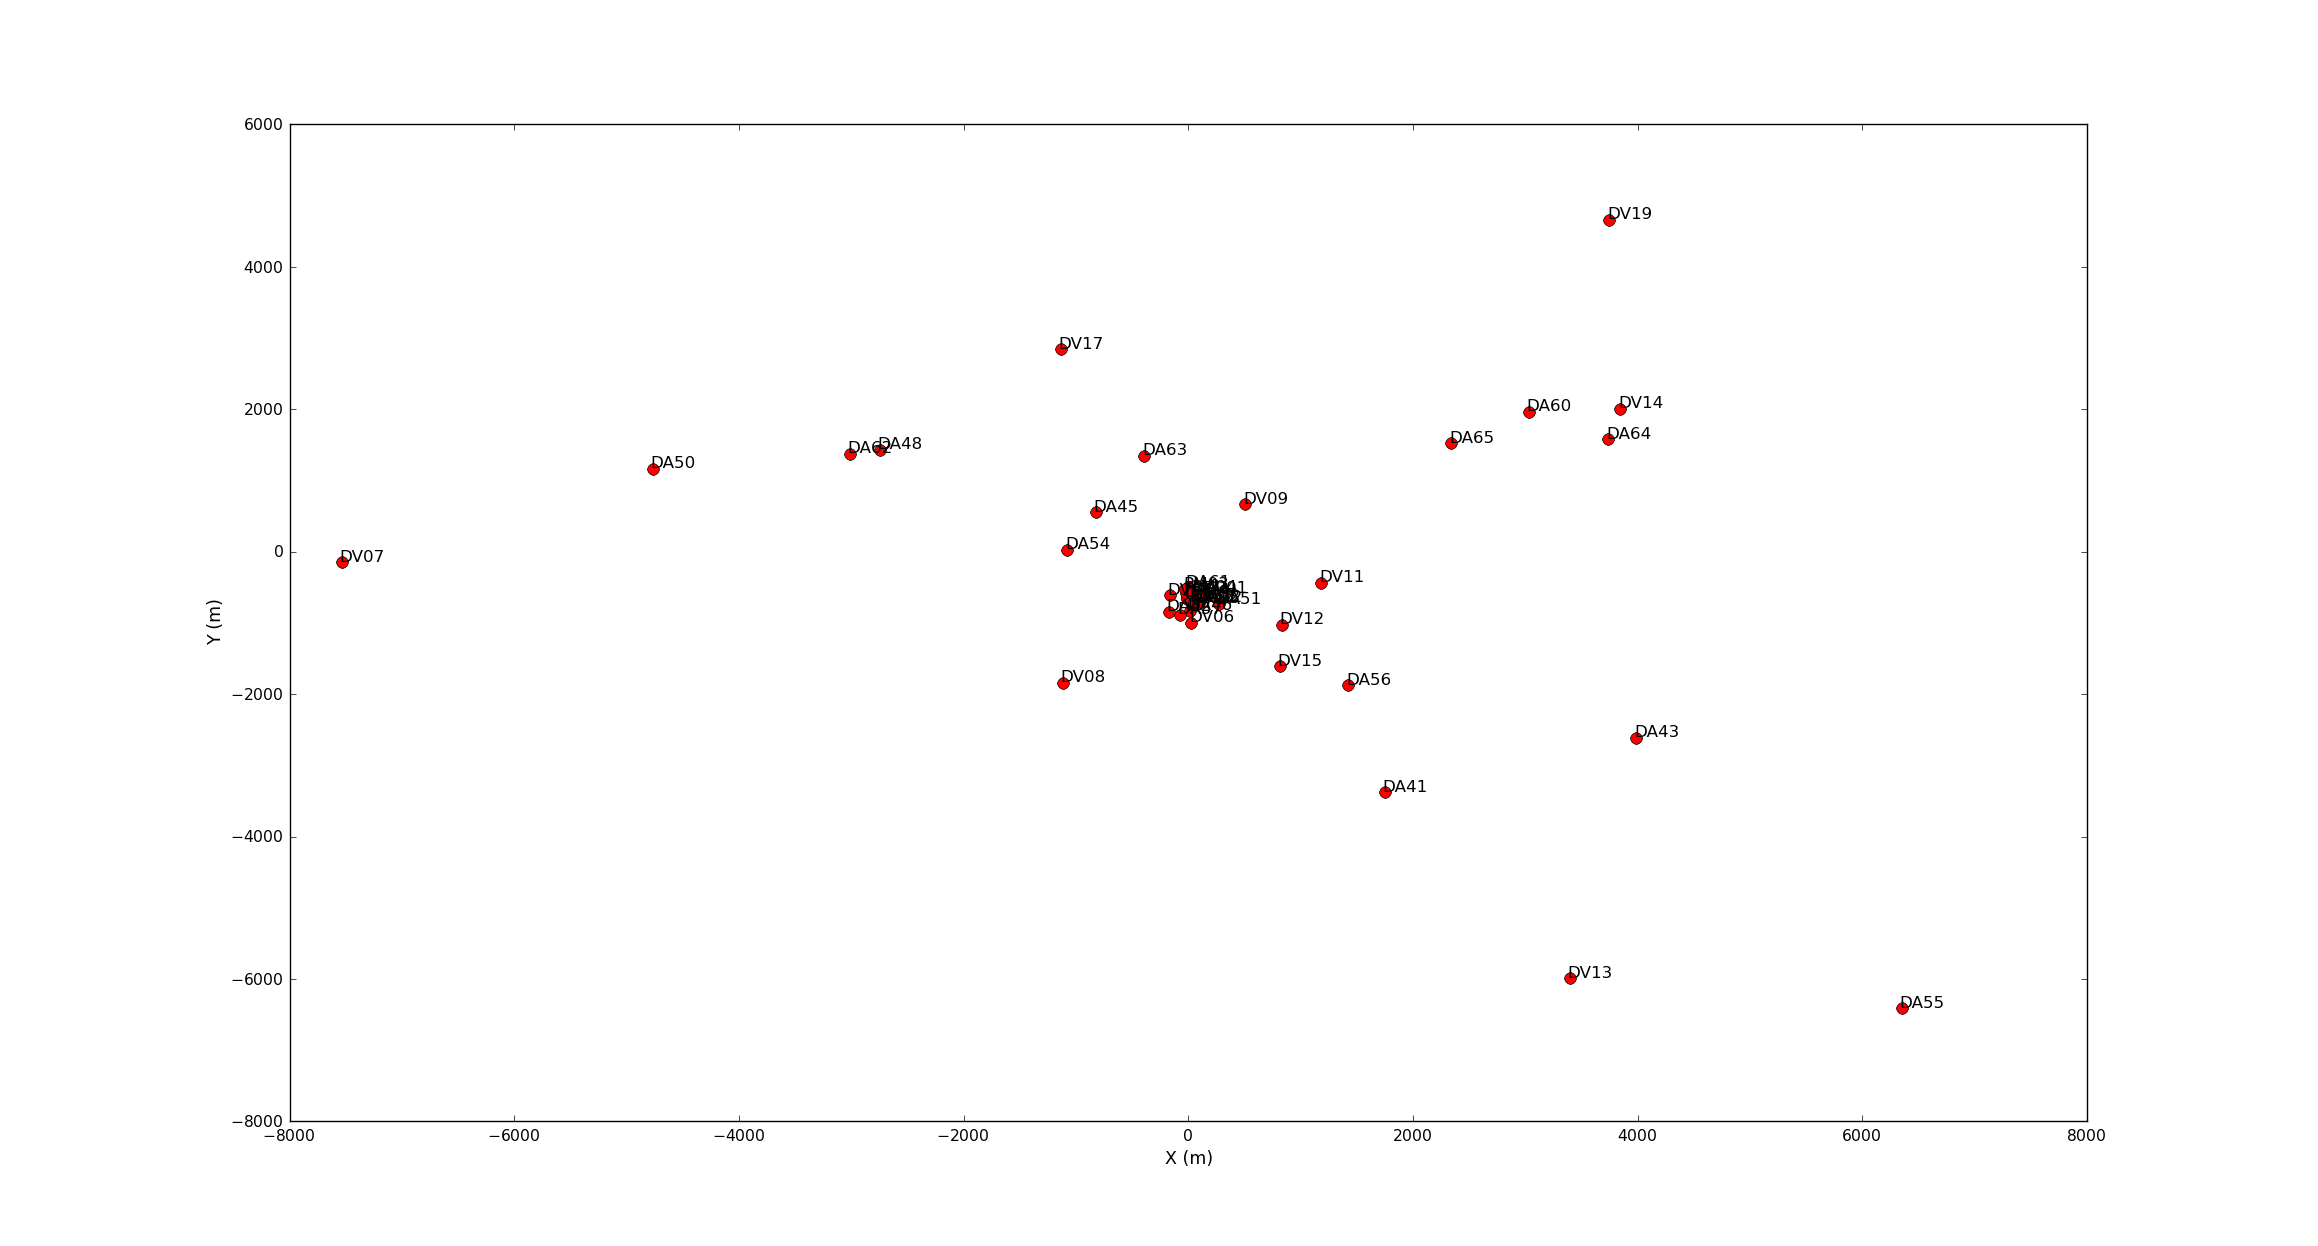
\includegraphics[scale=0.25]{images/HLTau_B6antennas1.png}
\caption{Distribución de antenas para el muestro del objeto HLTauri en banda 6. Fuente: Elaboración propia.}
\label{fig:almaarray1}
\end{figure}

\begin{figure}[h!]
\centering
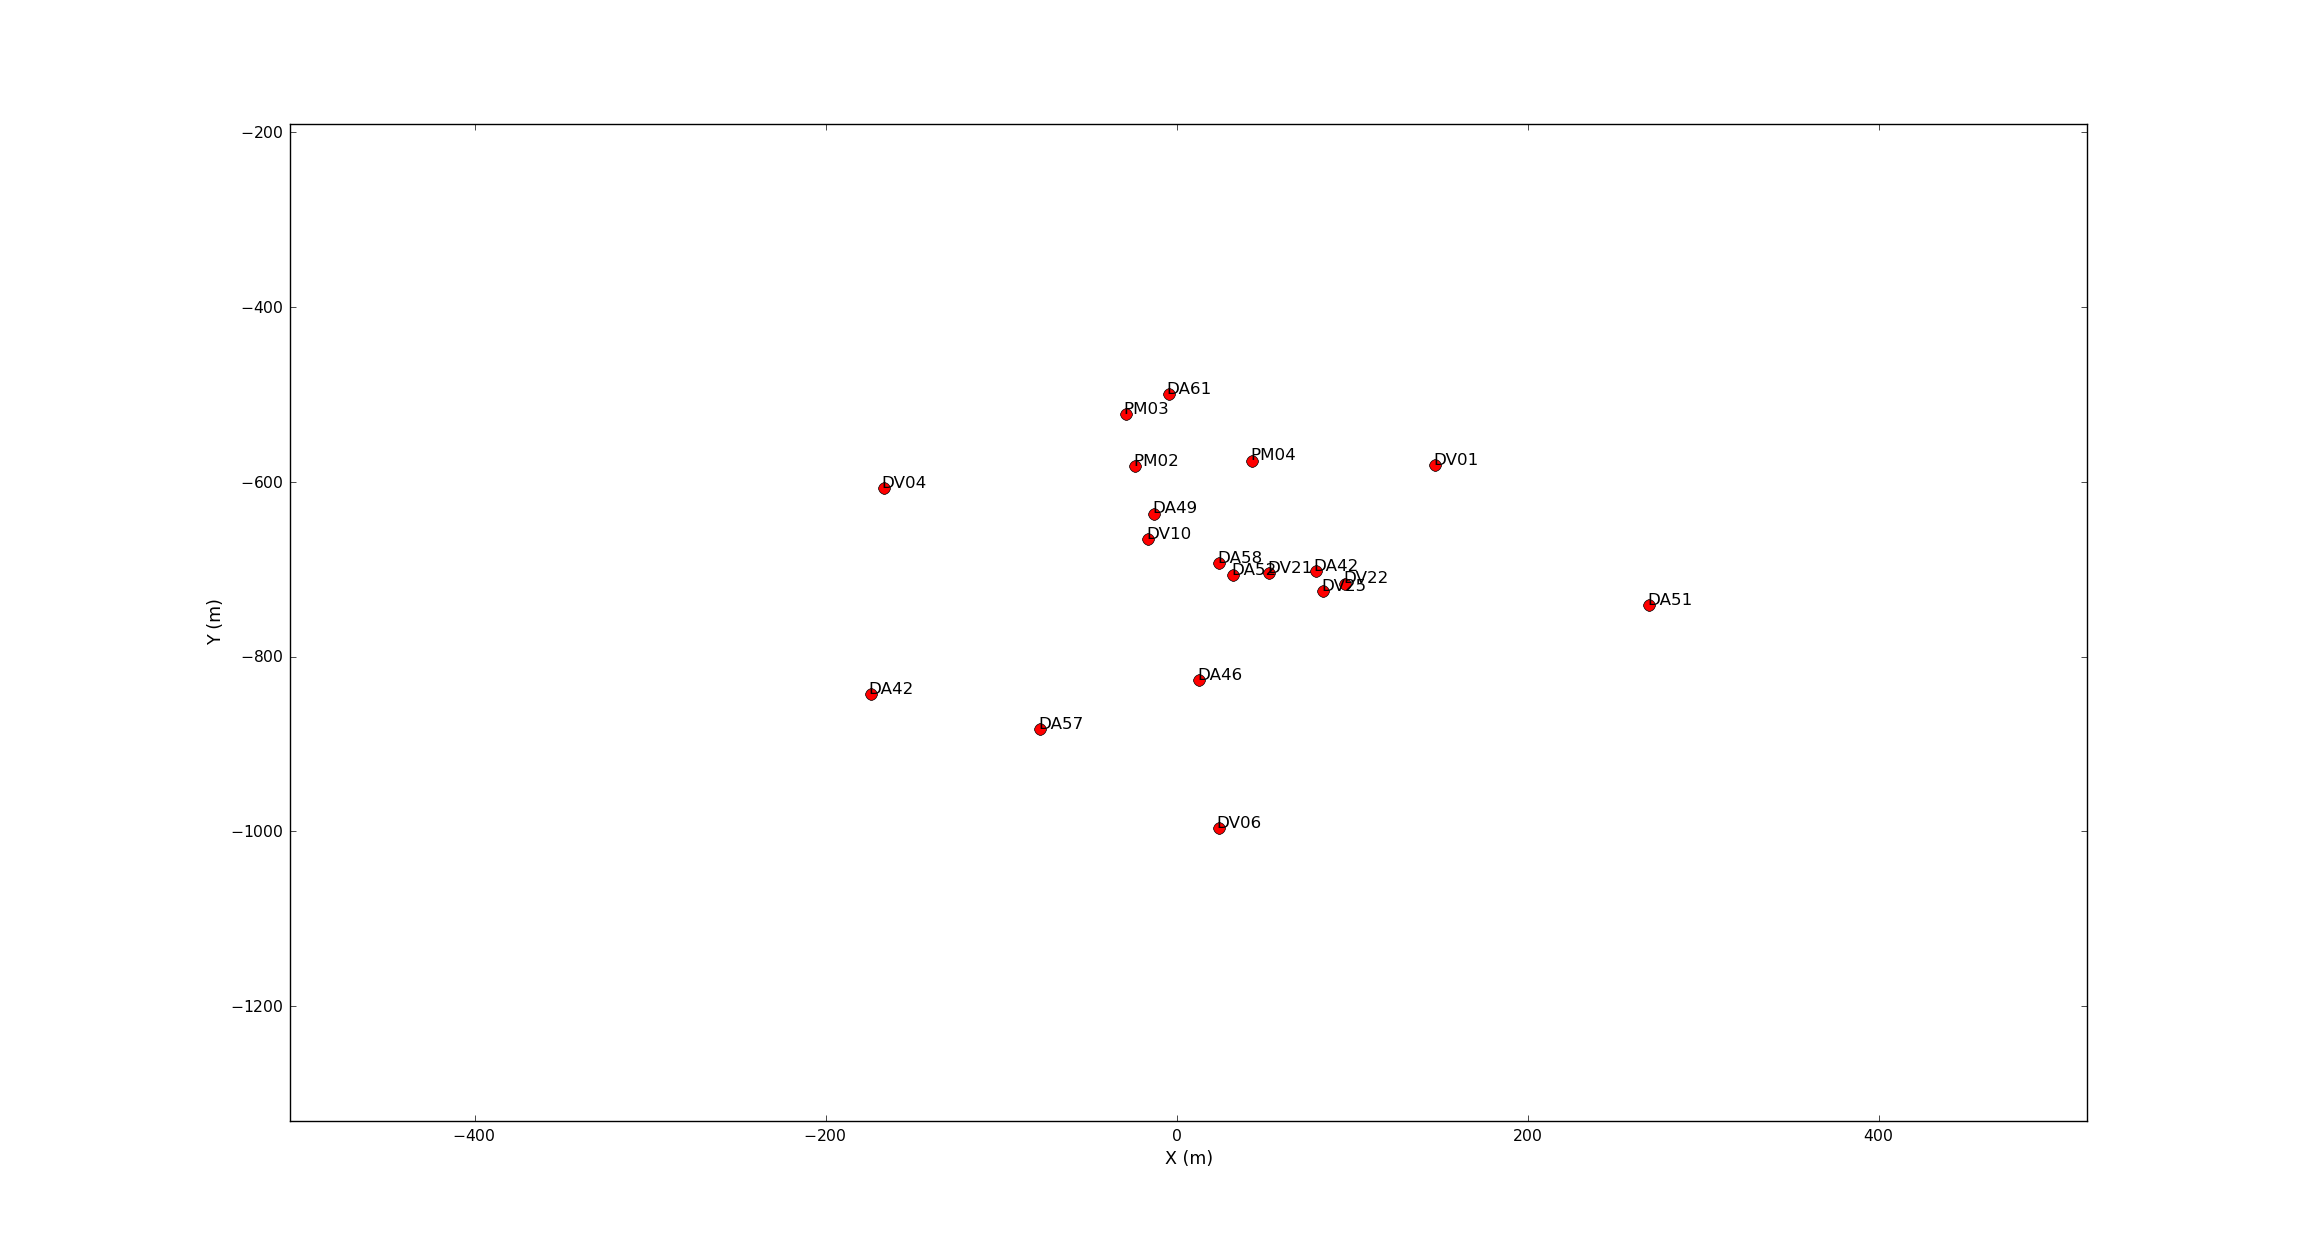
\includegraphics[scale=0.25]{images/HLTau_B6antennasCenter.png}
\caption{Centro de la distribución de antenas para el muestro del objeto HLTauri en banda 6. Fuente: Elaboración propia.}
\label{fig:almaarray2}
\end{figure}

Variados sistemas de coordenadas son usados para especificar la posiciones de las antenas en un \textit{array}. Uno de los sistemas usa coordenadas ecuatoriales horarias, es decir un ángulo horario $H$ y la declinación $\delta$. El ángulo $H$ se mide entre cero y 360 grados o entre cero y 24 horas sidéreas. Por lo tanto, a cada hora le corresponden $360°/24 = 15°$. Además, se mide a partir de la intersección del meridiano local con el ecuador. Su extremo es la intersección del meridiano que pasa por el objeto a observar ($S$) con el ecuador.

Por otra parte, la declinación es el ángulo medido sobre el meridiano que para por la estrella u objeto a observar, entre el ecuador la dirección de éste, sus valores están comprendidos entre cero y $+90°$ para los astros del hemisferio norte, y entre cero y $-90°$ para los astros del hemisferio sur \citep{astroelemental}.

En la Figura \ref{fig:ecuatorial2} se muestra el sistema de coordenadas ecuatoriales usado para arreglos de antenas terrestres. Se puede ver un sistema cartesiano donde $X$ e $Y$ están en un plano paralelo al ecuador de la tierra, donde $X$ es parte del plano meridiano (definido como el plano que pasa por los polos de la tierra y el punto de referencia del arreglo de antenas, $Y$ se mide hacia el este, y Z hacia el polo norte \citep{libroAstro}. En términos de ángulo horario $H$ y declinación $\delta$, las coordenadas $(X,Y,Z)$ se miden como lo muestra la Figura \ref{fig:ecuatorial1}.
%$H$ se mide a partir del punto $Q$ (intersección del meridiano del lugar con el Ecuador) en sentido horario. Su extremo es el punto $A$ (intersección del meridiano que pasa por el objeto a observar con el Ecuador). El ángulo $H$ se mide entre cero y 360 grados o entre cero y 24 horas sidéreas. Por lo tanto, a cada hora le corresponden $360°/24 = 15°$. Por otro lado, la declinación es el ángulo medido sobre el meridiano que pasa por la estrella u objeto a observar, entre el Ecuador y la dirección de éste. Es decir, el ángulo correspondiente al arco $AE$. Sus valores están comprendidos entre cero y $+90°$ para los astros del hemisferio Norte, y entre cero y $-90°$ para los astros del hemisferio Sur \citep{astroelemental}.
\begin{figure}[h!]
\centering
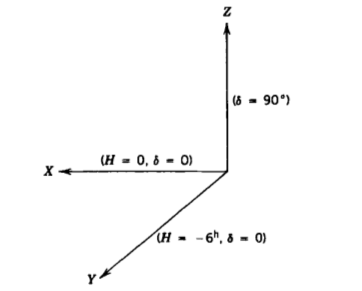
\includegraphics[scale=0.6]{images/ecuatorial1.png}
\caption{Sistema de coordenadas $(X,Y,Z)$ y la dirección de los ejes en términos de ángulo horario $H$ y declinación $\delta$. Fuente: \citep{libroAstro}}.
\label{fig:ecuatorial1}
\end{figure}

\begin{figure}[h!]
\centering
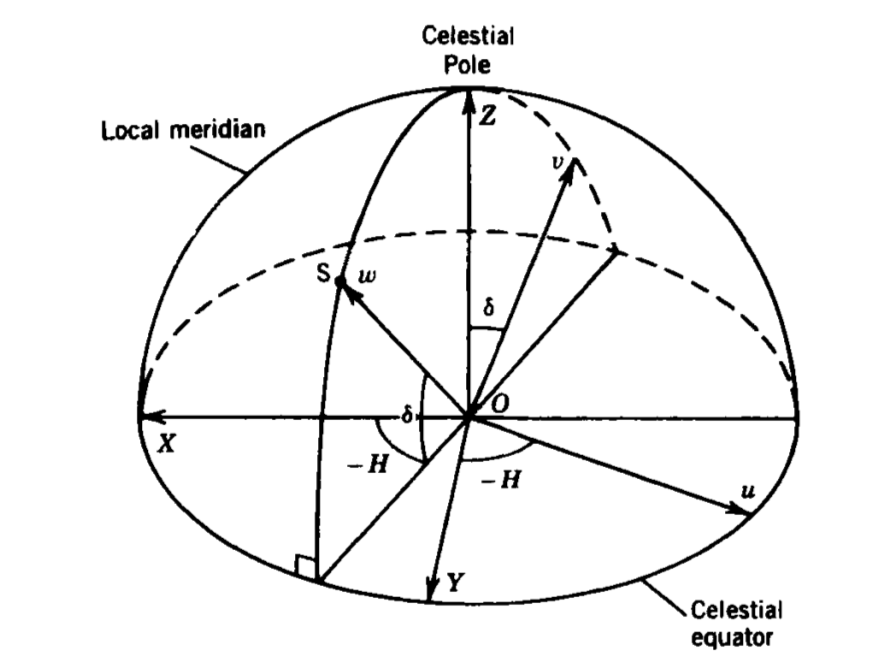
\includegraphics[scale=0.3]{images/ecuatorial2.png}
\caption{%Coordenadas ecuatoriales horarias.
Relación entre los sistemas de coordenadas $(X,Y,Z)$ y $(u,v,w)$. El sistema $(u,v,w)$ está definido por la observación en la dirección del punto $S$, el cual tiene un ángulo horario $H$ y una declicación $\delta$. Como $S$ está en el la mitad del hemisferio este, $H$ es negativo (sentido anti-horario). Fuente: \citep{libroAstro}}.
\label{fig:ecuatorial2}
\end{figure}

Es importante destacar que las estrellas describen en su movimiento diurno aparente, círculos paralelos de la Esfera Celeste y tienen por lo tanto declinación constante. Sin embargo, no sucede lo mismo con el Sol, la Luna o los planetas.

Teniendo esto en consideración, una coordenada del plano $(u,v)$ que genera un baseline está dada por:

\begin{equation}
\begin{bmatrix}
u\\
v\\
w
\end{bmatrix}
=
\begin{bmatrix}
\sin{H} & \cos{H} & 0\\
-\sin{\delta}\cos{H} & \sin{\delta}\sin{H} & \cos{\delta}\\
\cos{\delta}\cos{H} & -\cos{\delta}\sin{H} & \sin{\delta}
\end{bmatrix}
\begin{bmatrix}
X\\
Y\\
Z
\end{bmatrix}
\label{eq:uvw}
\end{equation}


Donde las coordenadas en el sistema $(X,Y,Z)$ están dadas por:

\begin{equation}
\begin{bmatrix}
X\\
Y\\
Z
\end{bmatrix}
=
D
\begin{bmatrix}
\cos{d}\cos{h}\\
-\cos{d}\sin{h}\\
\sin{d}
\end{bmatrix}
\label{eq:XYZ}
\end{equation}

Aquí, $(H, \delta)$ son el ángulo horario y la declinación de la posición de fase de referencia. Por otra parte es importante especificar el vector del \textit{baseline} en términos de su longitud $D$ y el ángulo horario y declinación $(h,d)$ de la intersección de la dirección del \textit{baseline} con el norte celestial. Reemplazando la Ecuación \ref{eq:XYZ} en \ref{eq:uvw} y usando identidades trigonométricas se tiene que:


\begin{equation}
\begin{bmatrix}
u\\
v\\
w
\end{bmatrix}
=
D
\begin{bmatrix}
\cos{d}\sin{(H-h)}\\
\sin{d}\cos{\delta}-\cos{d}\sin{\delta}\cos{(H-h)}\\
\sin{d}\sin{\delta}+\cos{d}\cos{\delta}\cos{(H-h)}
\end{bmatrix}
\label{eq:uvw2}
\end{equation}

Si bien el sistema $(D,h,d)$ era el más usado con instrumentos que sólo consistían en dos antenas. Cuando se tiene dos antenas o más, la práctica usual es utilizar el sistema de coordenadas horizontales para determinar la elevación $\mathscr{E}$, el \textit{azimuth} $\mathscr{A}$ y el largo del baseline $D$.

\begin{figure}[h!]
\centering
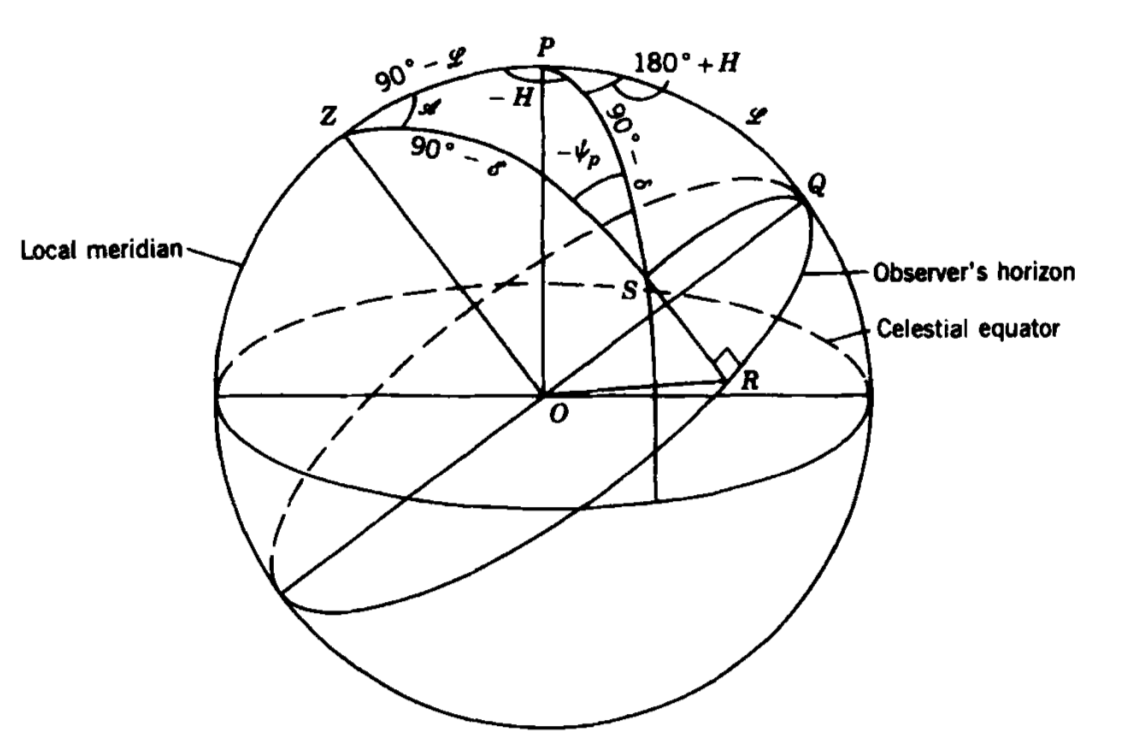
\includegraphics[scale=0.3]{images/horizontales.png}
\caption{Relación entre coordenadas horizontales y coordenadas ecuatoriales horarias. Fuente: \citep{libroAstro}}
\label{fig:horizontal}
\end{figure}

%%%%Explicar el sistema de coordenadas horizontales
El plano de referencia es el horizonte, perpendicular a la vertical del lugar de observación que pasa por el centro de la Tierra. $Z$ es el \textit{zenith} del observador y es la parte superior (más próximo al polo norte $P$) del plano vertical perpendicular al plano de observación. Por otra parte, el meridiano del lugar que pasa por el \textit{zenith}, corta al horizonte en una recta llamada meridiana que determina la dirección Norte-Sur. En este caso $Q$ indica el la dirección Norte, y luego mirando hacia éste, el Este queda a la derecha y el Oeste a la izquierda. Se llama \textit{azimuth} al ángulo $\mathscr{A}$ medido de Norte a Este en sentido anti-horario. Además, se llama elevación al ángulo $\mathscr{E}$ formado por la dirección de la fuente $S$ con el plano del horizonte.

Las fórmulas de conversión de coordenadas derivan de la aplicación de las reglas de seno y coseno para triángulos esféricos en la Figura \ref{fig:horizontal}. Por lo tanto para un observador a una latitud $\mathscr{L}$ se tiene que:

\begin{align}
\sin{d} &= \sin{\mathscr{L}}\sin{\mathscr{E}}+\cos{\mathscr{L}}\cos{\mathscr{E}}\cos{\mathscr{A}} \nonumber\\
\cos{d}\cos{h} &= \cos{\mathscr{L}}\sin{\mathscr{E}} - \sin{\mathscr{L}}\cos{\mathscr{E}}\cos{\mathscr{A}}\\
\cos{d}\sin{h} &= -\cos{\mathscr{E}}\sin{\mathscr{A}} \nonumber
\label{eq:transformation}
\end{align}

Reemplazando en la Ecuación \ref{eq:XYZ} se tiene:

\begin{equation}
\begin{bmatrix}
X\\
Y\\
Z
\end{bmatrix}
=
D
\begin{bmatrix}
\cos{\mathscr{L}}\sin{\mathscr{E}}-\sin{\mathscr{L}}\cos{\mathscr{E}}\cos{\mathscr{A}}\\
\cos{\mathscr{E}}\sin{\mathscr{A}}\\
\sin{\mathscr{L}}\sin{\mathscr{E}}+\cos{\mathscr{L}}\cos{\mathscr{E}}\cos{\mathscr{A}}
\end{bmatrix}
\end{equation}


Por otra parte, si se quisiera proyectar el plano $(u,v)$ en la Figura \ref{fig:ecuatorial2} bastaría que hicieramos $H=0$ en la ecuación \ref{eq:uvw} o \ref{eq:uvw2}, con esto se forma una ecuación de la elipse en el plano $(u,v)$ de la forma:

\begin{equation}
\frac{u^2}{(\sqrt{X^{2}+Y^{2}})^2}+\frac{(v-Z\cos{\delta})^2}{(\sin{\delta}\sqrt{X^{2}+Y^{2}})^2} = 1
\label{eq:elipse}
\end{equation}

Si se analiza la ecuación \ref{eq:elipse} es posible notar que su centro está en $(u,v)=(0,Z\cos{\delta})$, su eje semimayor se encuentra en $\sqrt{X^{2}+Y^{2}}$ y su eje semimenor en $\sin{\delta}\sqrt{X^{2}+Y^{2}}$. Este arco trazado durante la observación depende del \textit{azimuth}, la elevación y la latitud del \textit{baseline}; la declinación de la fuente, y el rango de ángulo horario que se cubre como se muestra en la Figura \ref{fig:uvplane2}. Además, como una de las propiedades de la transformada de Fourier es la simetría Hermitiana $V(u,v)=V(-u,-v)$, el correlacionador devuelve como salida el valor de la visibilidad en dos puntos en el plano $(u,v)$ como se muestra en la Figura \ref{fig:uvplane1}.

\begin{figure}[h!]
\centering
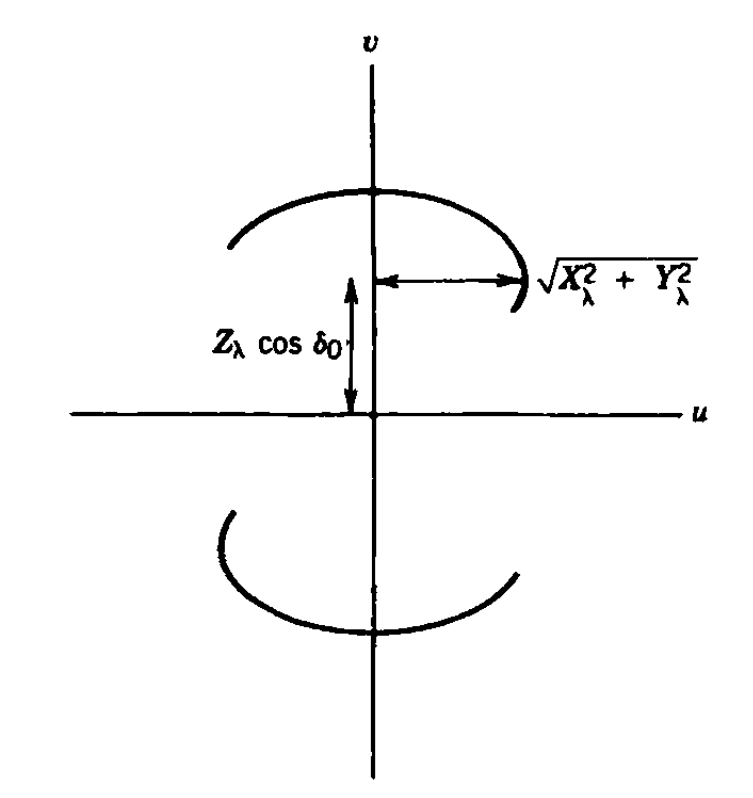
\includegraphics[scale=0.3]{images/uvplane1.png}
\caption{Centro y eje semimayor de la elipse (Ecuación \ref{eq:elipse}). Fuente: \citep{libroAstro}}
\label{fig:uvplane1}
\end{figure}

\begin{figure}[h!]
\centering
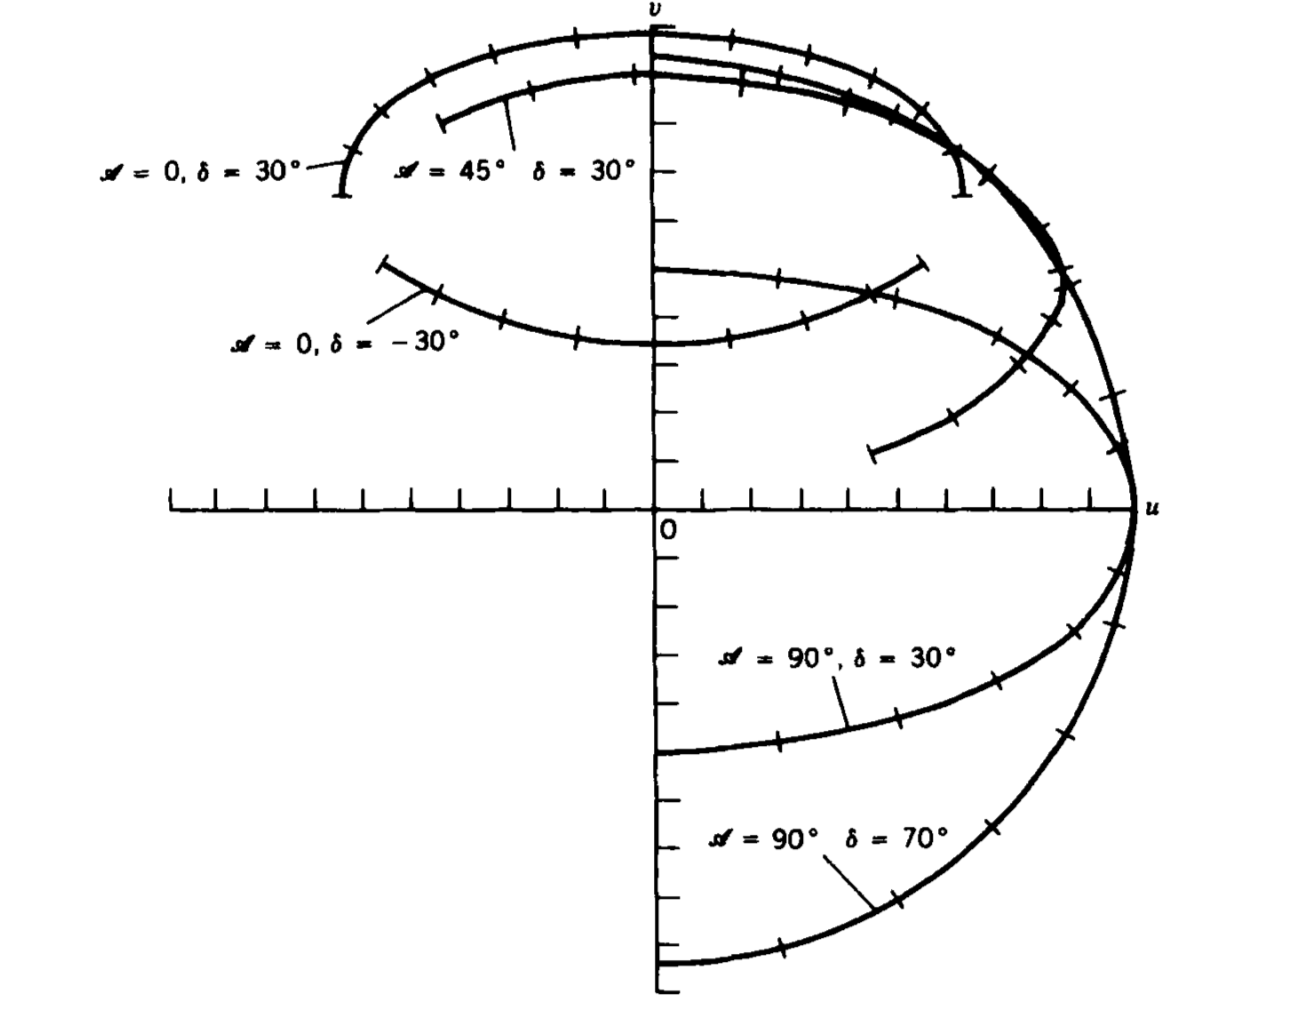
\includegraphics[scale=0.3]{images/uvplane2.png}
\caption{Elipses muestreadas con diferentes parámetros en el plano $(u,v)$. Fuente: \citep{libroAstro}}
\label{fig:uvplane2}
\end{figure}



\clearpage

Por otro lado, cada antena contiene un receptor (también llamado \textit{Front-end}) que permite que las éstas capten información en diez bandas de frecuencia diferentes. Para ello cada antena está equipada con un criostato y su criorefrigerador adjunto. Estos criostatos contienen receptores que están montados y pueden ser reemplazados de forma fácil. En la tabla \ref{tab:bands} se adjuntan los datos de las distintas bandas de frecuencia que ALMA puede cubrir gracias a su front-end.


\begin{table}[h!]
\centering
\ra{1.2}
\begin{tabular}{@{}rcrrcr@{}}
\toprule
 \multicolumn{1}{c}{{\bf Banda}} & \phantom{a} & \multicolumn{2}{c}{{\bf Rango de frecuencia (GHz)}}  & \multicolumn{1}{c}{{\bf Temperatura (K)}} \\
 \midrule
 1   && 31 - 45 &&  26\\
 2   && 67 - 90 &&  47\\
 3  && 84 - 116 &&  60\\
 4  && 125 - 163 &&  82\\
 5  && 162 - 211 &&  105\\
 6  && 211 - 275 &&  136\\
 7  && 275 - 373 &&  219\\
 8  && 385 - 500 &&  292\\
 9  && 602 - 720 &&  261\\
 10  && 787 - 950 &&  344\\
 \toprule
\end{tabular}
\caption{Las 10 Bandas de frecuencia de ALMA}
\label{tab:bands}
\end{table}

Por ejemplo, la estrella HLTauri ha sido muestreada en las bandas 3, 6 y 7. En la Figura \ref{fig:HLTau-total} es posible apreciar cada uno de los planos $(u,v)$ formados en cada muestreo.


\begin{figure}[h!]
\centering
\subfloat[Banda 3]{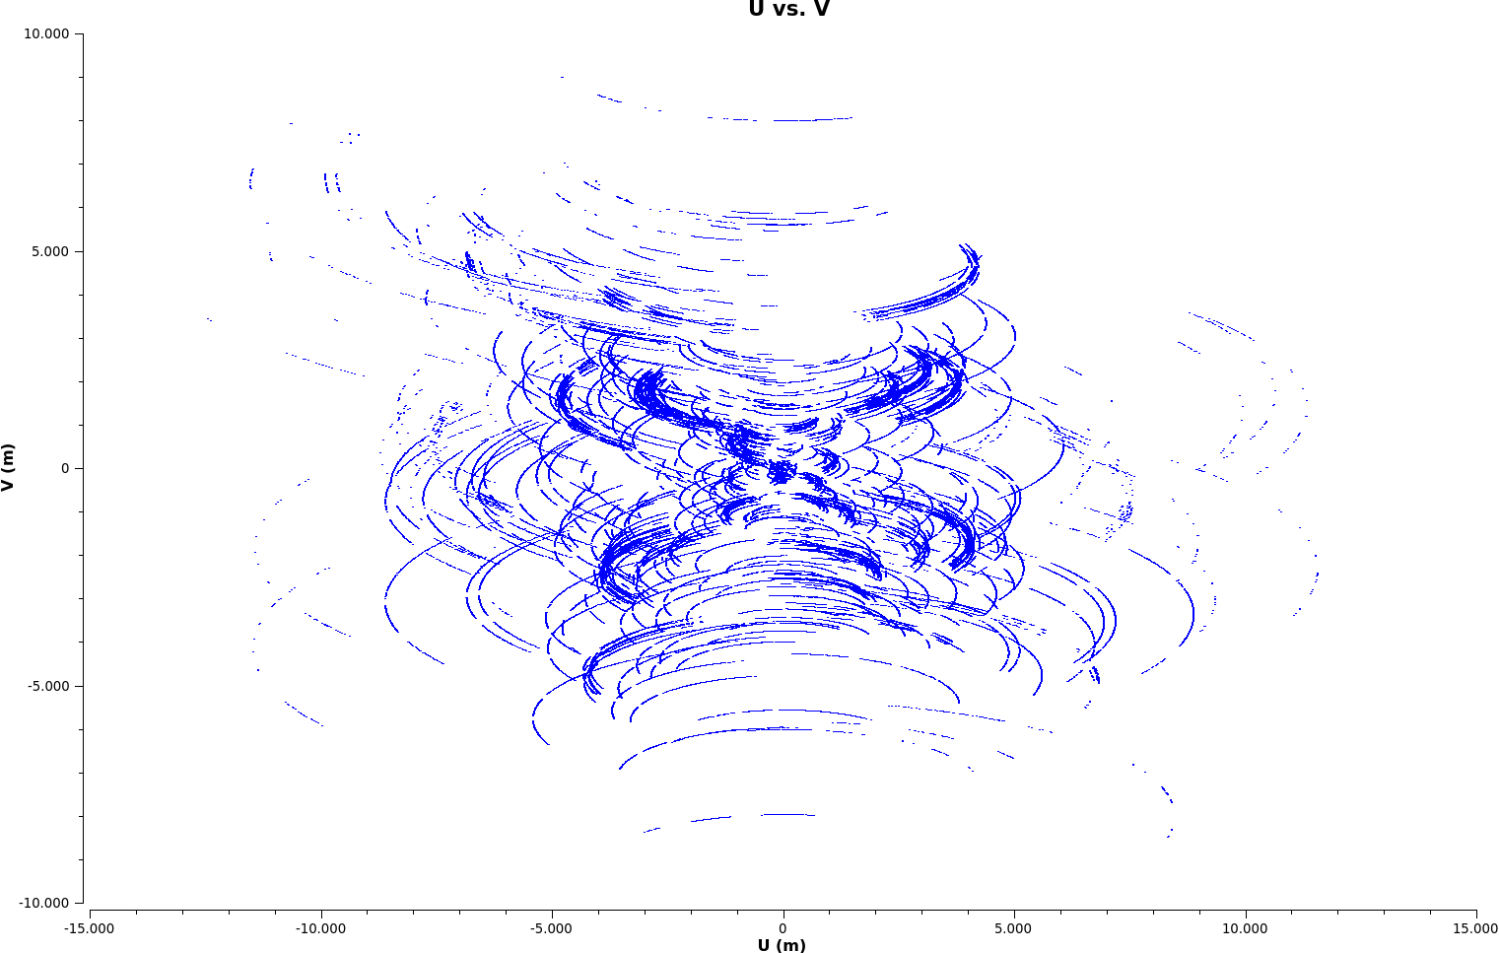
\includegraphics[scale=0.15]{images/HLTau_B3total.png}}%
\subfloat[Banda 6]{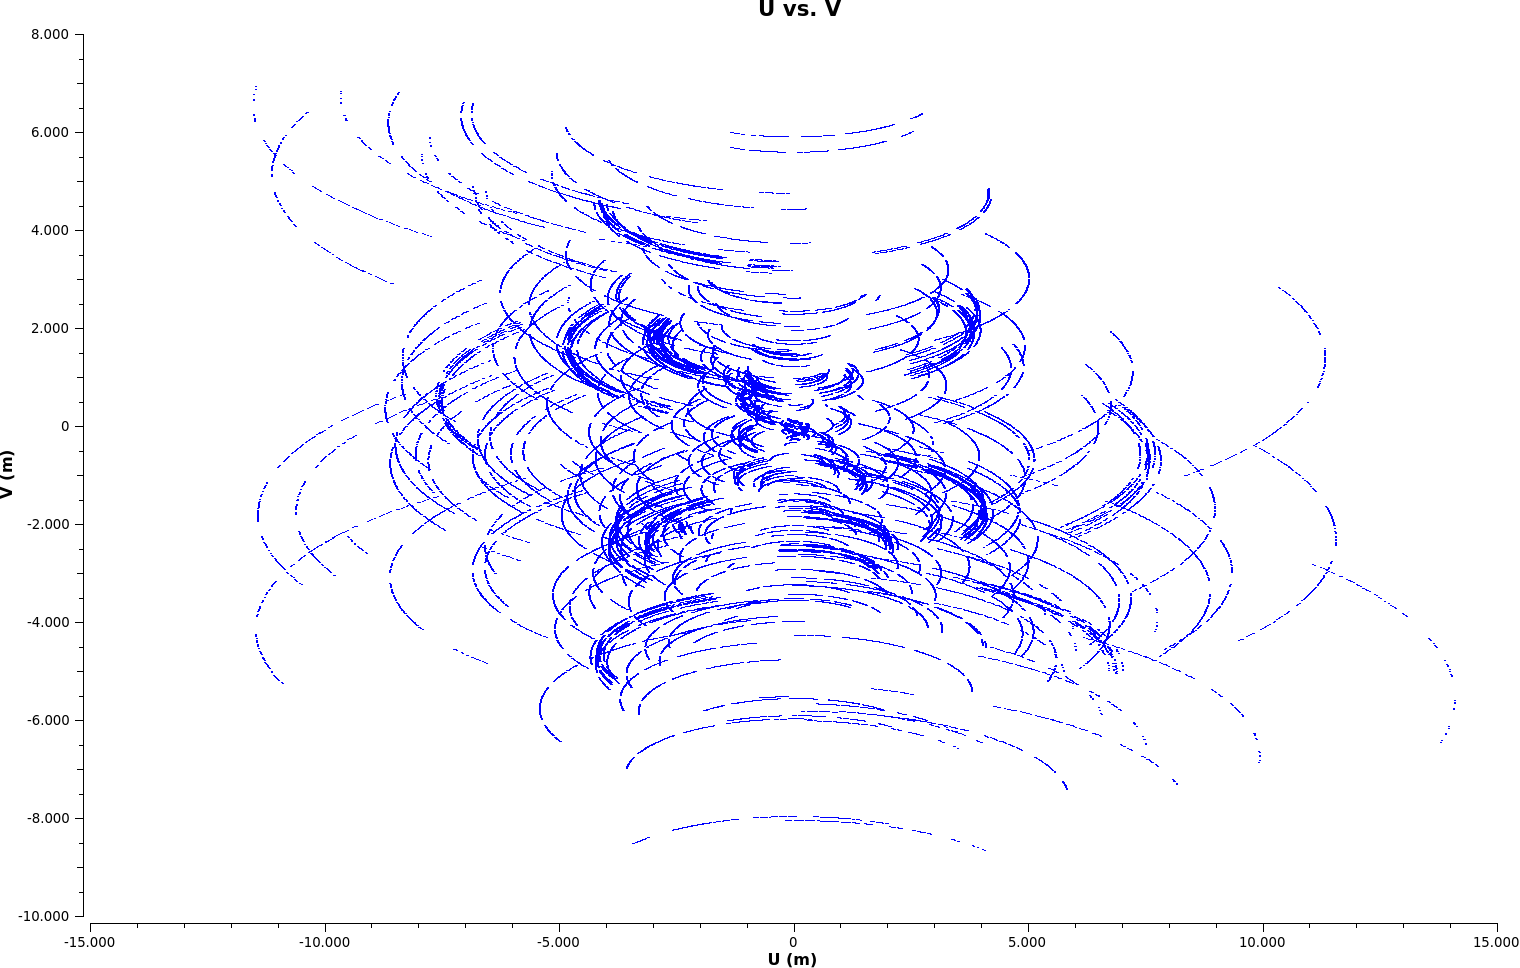
\includegraphics[scale=0.15]{images/HLTau_B6total.png}}\\
\subfloat[Banda 7]{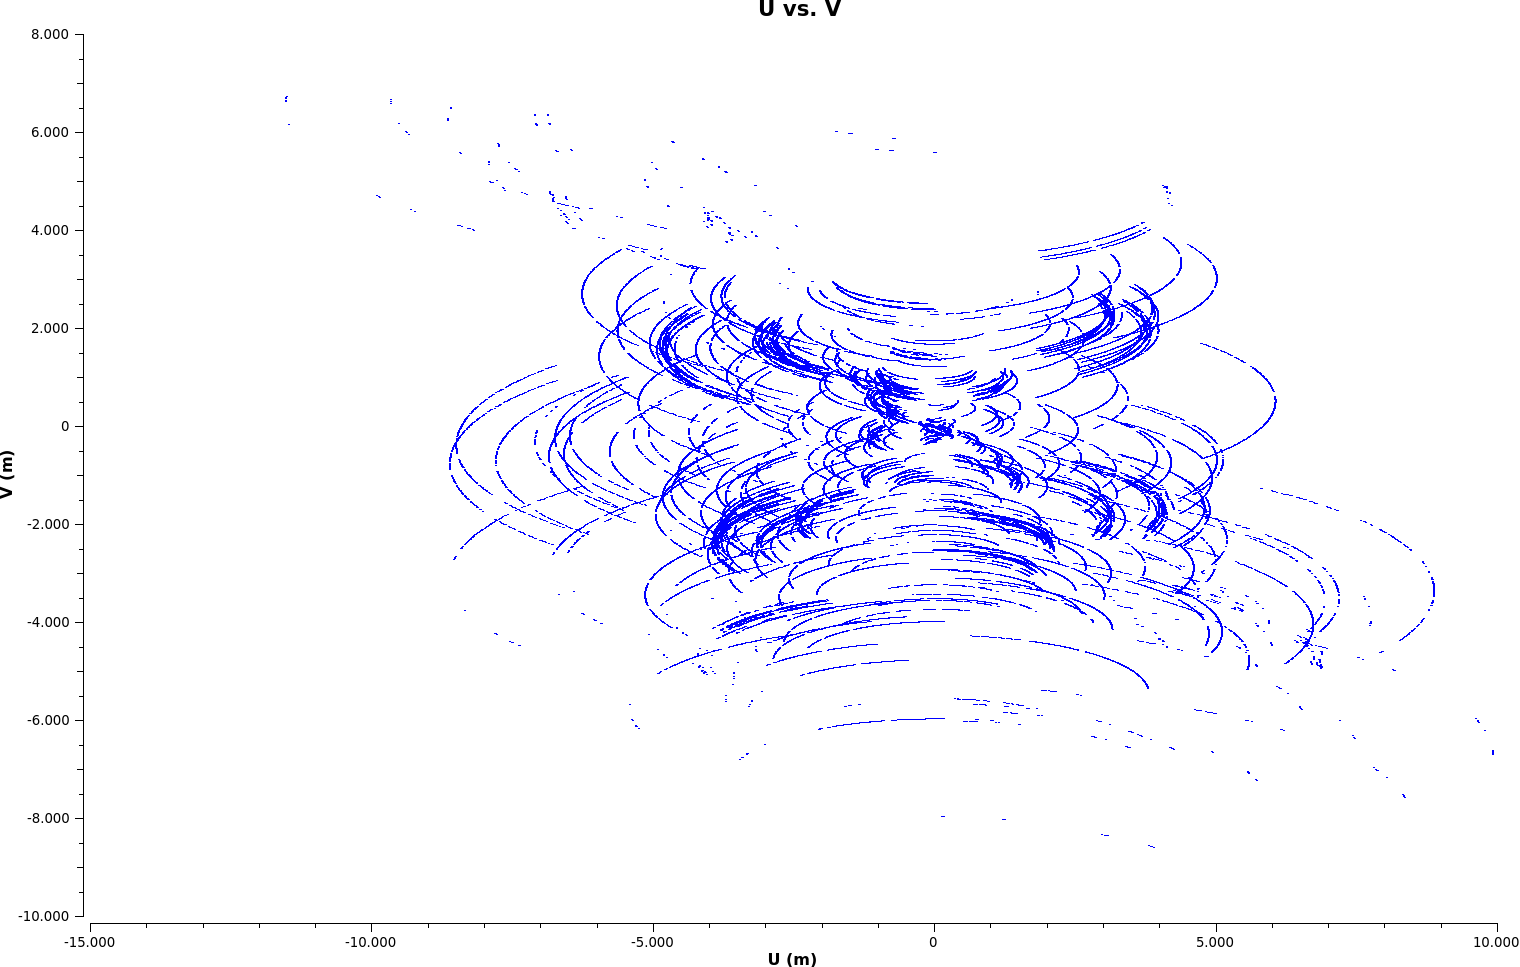
\includegraphics[scale=0.15]{images/HLTau_B7total.png}}%
\caption{Plano $(u,v)$ del objeto HLTauri (HLTau) en diferentes bandas. Fuente: Elaboración propia}
\label{fig:HLTau-total}
\end{figure}

Es importante destacar que los datos muestreados en una banda se separan en \textit{spectral windows} que son espectros contiguos cuyas frecuencia están uniformemente espaciadas con anchos de banda desde 58.6 MHz hasta 1.875 GHz \citep{alma-handbook}. Asimismo, cada \textit{spectral window} se divide uniformemente en canales. Es posible visualizar esto en la Figura \ref{fig:division}, en donde se ha puesto como ejemplo el muestreo del objeto HL-Tauri.

\begin{figure}[h!]
\centering
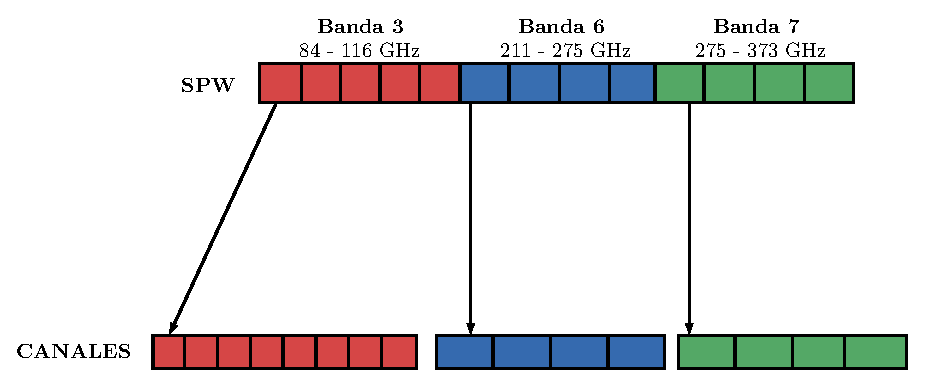
\includegraphics[scale=0.8]{images/frecuencias.eps}
\caption{Bandas, \textit{spectral windows} y canales del objeto HL-Tauri. Fuente: Elaboración propia}
\label{fig:division}
\end{figure}




Luego de que las ondas milimétricas y submilímetricas son recibidas por las antenas, éstas deben ser discretizadas y procesadas en uno de los dos correlacionadores. El correlacionador \textit{64-input} es usado principalmente por los conjuntos de antena de 12 metros, mientras que el correlacionador ACA es usado por las antenas de 7 metros que componen el \textit{Atacama Compact Array}. Así, ambos correlacionadores funcionan simultáneamente e independientemente, por lo que mientras las antenas de 12 metros pueden estar observando un objeto y usan el correlacionador \textit{64-input}, las antenas de 7 metros pueden estar observando el mismo y otro objeto, y además, usando el correlacionador ACA \citep{alma-handbook}.

Es importante destacar que los correlacionadores reciben señales de voltaje desde cada antena, calculan la correlación cruzada y autocorrelación para éstas por cada par de antenas (\textit{baselines}), y producen las visibilidades de valores complejos que los astrónomos reciben para sintetizar imágenes. Para entender de mejor forma qué son las visibilidades y cual es la implicancia que tienen en la síntesis de imágenes es necesario conocer los conceptos esenciales de interferometría.

\section{Principios y conceptos de interferometría}

La interferometría es una técnica usada para obtener imágenes de alta resolución angular de un fenómeno astronómico particular. Esta implica la combinación de señales recibidas desde el cielo por dos antenas separadas físicamente. Estas señales contienen ruido, permitiendo así que la distribución del brillo del cielo sea muestreada en una escala angular más pequeña que la de una sola antena.

La resolución angular de un interferómetro, $\delta$, es el ángulo más pequeño en el que dos objetos pueden ser separados en orden de distinguirlos como objetos diferentes. Usando la teoría de la difracción, se puede demostrar que que para un interferómetro circular en particular de diámetro $D$, y una radiación de longitud de onda $\lambda$, este valor es $\delta \propto \frac{\lambda}{D}$. Esto quiere decir, que para grandes longitudes de onda (pequeñas frecuencias), se necesita un gran telescopio para obtener una buena resolución. Sin embargo, existen límites prácticos para construir un telescopio de un gran tamaño. Es por ello que haciendo uso de un conjunto de interferómetros situados a una distancia $D$, es posible obtener la misma resolución que un solo telescopio de radio $D$.



La relación entre la distribución del brillo del cielo y una visibilidad compleja está dada por el teorema de van Cittert-Zernike \citep{zernike} y es la base de la interferometría. Dado que los interferómetros no obtienen la imagen del cielo directamente, sino que obtienen visibilidades, que son que son la transformada de Fourier de la distribución del brillo del cielo en el plano de la imagen. Cada par de antenas forma un vector $\vec{k} = (u,v)$ en el plano de Fourier. Así mismo, la distribución del brillo del cielo es la transformada inversa de Fourier de las visibilidades complejas. Por lo tanto, la visibilidad $V(\vec{k})$ para un par de antenas con un \textit{baseline} $\vec{k}$, y su respectiva transformada inversa es:

%\begin{equation}
%V(\vec{k}) = \int_{-\infty}^{+\infty} A(\vec{x})I(\vec{x})e^{2\pi i %\vec{k}\vec{x}}\frac{dx dy}{\sqrt{1-x^{2}-y^{2}}}
%\end{equation}

\begin{align}
V(\vec{k}) &= \int\int A(\vec{x})I(\vec{x})e^{-2\pi i\vec{k}\vec{x}}dxdy \\
A(\vec{x})I(\vec{x}) &= \int\int V(\vec{k})e^{2\pi i\vec{k}\vec{x}}dudv
\end{align}

Donde $\vec{x} = (x,y)$ son las coordenadas del objeto a observar y estudiar, $A(\vec{x})$ es el \textit{primary beam}, $I(\vec{x})$ es la intensidad del objeto en $\vec{x}$, y $\vec{k}$ es el vector que se forma por cada par de antenas.

\begin{figure}[h!]
\centering
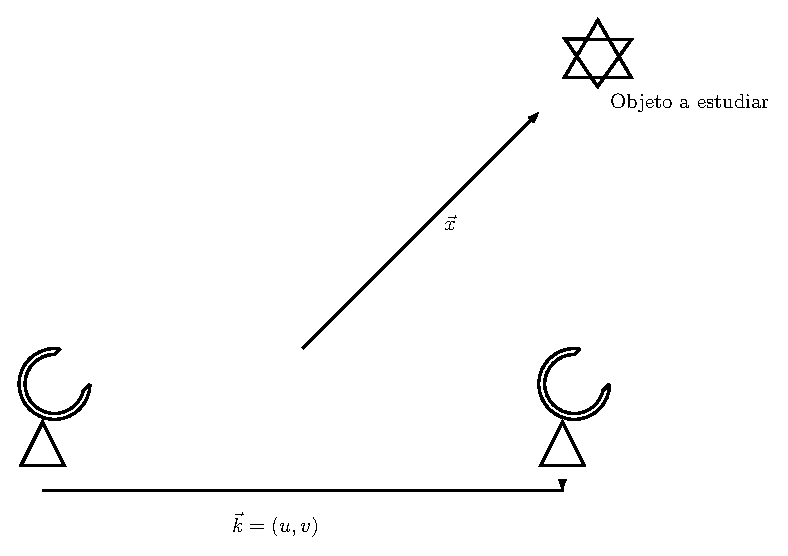
\includegraphics[scale=0.7]{images/antenas.eps}
\caption{Dos antenas y su respectivo \textit{baseline}. $\vec{x}$ es la posición del objeto estudiado, y por otro lado $\vec{k}$ es el \textit{baseline} correspondiente a las dos antenas. Fuente: Elaboración propia.}
\label{fig:antena}
\end{figure}

Esto quiere decir que la imagen de la distribución del brillo del cielo puede recuperarse a través del muestreo de la distribución de visibilidades complejas en el plano $(u,v)$. En esencia, una imagen es la transformada de Fourier de las visibilidades donde cada una de éstas tiene una amplitud y una fase representando el brillo y la posición relativa de la emisión en una escala angular específica.

%Debido a que existe un número finito de pares de antenas, al llevar a cabo una transformada de Fourier inversa aparecen \textit{side-lobes} rodeando al \textit{primary beam}. Los \textit{side-lobes} son irregularidades en los patrones de radiación debido a la extensión finita de los puntos en el plano $(u,v)$ y a deficiencias en la cobertura. La transformada inversa de Fourier aplicada a las visibilidades es llamada \textit{dirty map}. El \textit{dirty map} ($I_{D}$) es la imagen del cielo ($I_{sky}$) convolucionada con el \textit{beam} del interferómetro ($B$).

%\begin{equation}
%I_{D} = I_{sky} \ast B
%\end{equation}

%El \textit{beam} $B$ para un interferómetro con un conjunto de \textit{baselines} $\{\vec{k}_{k}\}$ puede ser representado por la transformada inversa de Fourier de una suma de diferencias en estos puntos en el plano $(u,v)$.

%\begin{align}
%B(\vec{x}) &= \int_{-\infty}^{+\infty}\sum_{k}\delta(\vec{k}-\vec{k}_{k})e^{2 \pi i \vec{k}_{k}\vec{x}}dudv \\
%&= \sum_{k}\left(\cos(-2\pi\vec{k}_{k}\vec{x})+i\sin(-2\pi\vec{k}_{k}\vec{x})\right) \\
%&= \sum_{k}\cos(2\pi\vec{k}_{k}\vec{x})
%\end{align}


Los datos astronómicos resultan desde la adición de el ruido instrumental hasta la convolución de la imagen del cielo con la respuesta instrumental. Debido al muestreo incompleto en el plano $(u,v)$, la obtención de una imagen del cielo se convierte en un problema inverso que requiere algoritmos de síntesis de imágenes.


\section{Métodos existentes de deconvolución}

\subsection{CLEAN}

Uno de los algoritmos más exitosos y utilizados por la comunidad astronómica es CLEAN, creado por \citep{hogbom}. CLEAN postula que la distribución de intensidad está compuesta de fuentes puntuales. Dado que la imagen de una fuente puntual está dada por la convolución de ésta con el \textit{dirty beam} o Point Spread Function (PSF) (Ecuación \ref{eq:dirtybeam}). Donde este último está dado por:

\begin{equation}
B(x,y) = \int\int S(u,v) \exp\{2\pi j(ux+vy)\} \;du\,dv
\label{eq:dirtybeam}
\end{equation}

En cada iteración CLEAN encuentra el punto más brillante en la \textit{dirty image} (Ecuación \ref{eq:dirtyimage}) que está dada por:

\begin{equation}
I_{D}(x,y) = \int\int V(u,v)S(u,v)e^{2\pi i(ux+vy)}\;du\,dv
\label{eq:dirtyimage}
\end{equation}

Donde,

\begin{equation}
I^{T}(x,y) = \int\int V(u,v)e^{2\pi i(ux+vy)}\;du\,dv
\label{eq:fullcoverage}
\end{equation}

Y luego por el teorema de la convolución se tiene que:

\begin{equation}
I_{D}(x,y) = I^{T}(x,y) \ast B(x,y)
\end{equation}

CLEAN agrega este punto (posición e intensidad) a la lista de fuentes puntuales. Luego, una fracción de ésta ($\gamma$, $0 < \gamma < 1$) es removida de la \textit{dirty image} y de las visibilidades. Este proceso se repite hasta que la imagen residual ($I_D$) sea solamente ruido.

Finalmente se calcula la imagen reconstruida convolucionando la lista de fuentes puntuales con el \textit{beam} de CLEAN, que se asume la mayoría de las veces como una Gaussiana.

\begin{algorithm}
\begin{algorithmic}[1]
    \STATE{Compute $I_D(x,y)$}
    \STATE{$B_R(x,y) = Gaussian$}
    \STATE{$i=0$}
    \WHILE{$I_D$ not noise-like}
        \STATE{$(x_i, y_i) = \arg\max I^D(x,y)$}
        \STATE{$\lambda_i = I(x_i, y_i)$}
        \FORALL{$(u,v)$}
            \STATE{$V(u,v) -= \gamma \lambda_i \exp\{-2\pi j(u x_i+ v y_i)\}$}
        \ENDFOR
        \STATE{Recompute $I_D(x,y)$}
        \STATE{$i=i+1$}
    \ENDWHILE
    \STATE{$I_R(x,y) = I_D(x,y) + \sum_i \gamma\lambda_i B_R(x-x_i,y-y_i)$}
\end{algorithmic}
\label{alg:clean}
\caption{Algoritmo CLEAN}
\end{algorithm}


\subsection{MEM Mono-frecuencia}


El método de máxima entropía (MEM) encuentra la imagen que simultáneamente se ajuste mejor a los datos, dentro de un nivel de ruido y que maximice la entropía $S$. Esto se lleva a cabo minimizando la función:

En MEM, la imagen y los datos son considerados variables aleatorias con distribuciones de probabilidad conocidas.

Sea $P(V|I)$ la probabilidad de ver las visibilidades $V$ dada la imagen $I$ y sea $P(I)$ un conocimiento \textit{a priori} de la imagen. Entonces mediante el teorema de Bayes se obtiene:

\begin{equation}
P(I|V) = \frac{P(V|I)P(I)}{P(V)}
\label{eq:bayes}
\end{equation}

La probabilidad $P(V|I)$ puede ser aproximada mediante el hecho de que las visibilidades están corruptas por un ruido Gaussiano. Entonces dada la función modelo de visibilidades $V_{k}^{m}(I)$ y las varianzas observadas $\sigma_k$, la probabilidad puede modelarse como lo muestra la ecuación \ref{eq:chi2}, donde $V_{k}^{o}$ son las visibilidades observadas.

\begin{equation}
 P(V|I) \propto \exp\biggl\{-\sum_j^{Z}{\frac{|V^m_j(I)-V^o_j|^{2}}{\sigma_j^{2}}}\biggr\}
 \label{eq:chi2}
\end{equation}

El \textit{prior} $P(I)$ se considera una distribución multinomial de una intensidad total discreta que cubre la imagen completa. Sea $n$ el número de píxeles y sea $N_{i}$ el número de fotones en el píxel $i$, el \textit{prior} puede expresarse de la forma:

\begin{equation}
P(I) = \frac{N!}{n^N\prod_i{N_i!}}
\label{eq:imageProb}
\end{equation}

Donde $N=\sum_i N_{i}$ y la intensidad de la imagen en el píxel $i$ es interpretado en el modelo como $I_{i} \propto N_{i}$.

El término $P(V)$ en la ecuación \ref{eq:bayes} es independiente de $I$, por lo tanto no forma parte de la ecuación. Usando logaritmo y la aproximación de Stirling para factoriales y además omitiendo constantes aditivas relevantes el problema de reconstrucción de la imagen se convierte en la búsqueda de una imagen que satisfaga la probabilidad Maximum a Posteriori (MAP).

\begin{equation}
\arg \max_{I} \biggl\{
            -\frac{1}{2} \sum_j^{Z}{ \frac{|V^m_j(I)-V^o_j|^{2}}{\sigma_j^2} }-
            \lambda \sum_k^{n}{I_k \log{\frac{I_k}{G}}}
            \biggr\}
\label{eq:phi}
\end{equation}

Se reconoce al primer término de la ecuación \ref{eq:phi} como $\chi^{2}$ y al segundo como la entropía de Shannon $S$. Estos dos parámetros son relevantes en el modelo, así como $\lambda$ que tiene un rol similar a los multiplicadores de Lagrange y actúa como un penalizador.

Finalmente, se cambia el signo de la ecuación \ref{eq:phi}, convirtiendo el problema en una minimización.

\begin{align}
\label{eq:phiFinal}
 \Phi = \frac{1}{2}\sum_j^{Z}{{\frac{|V^m_j(I)-V^o_j|^2}{\sigma_j^2}} + \lambda \sum_k^{n}{I_k \log{\frac{I_k}{G}}}}
\end{align}


Note que la Ecuación \ref{eq:phiFinal} es no lineal, por lo que debe ser minimizada con los algoritmos apropiados, en el caso de la solución que se propone, el método usado es el del gradiente conjugado Polak-Ribiere \citep{polak}. Además, es importante destacar que esta ecuación asume la existencia de un \textit{spectral window} y un solo canal.

En el Anexo \ref{apendice:dphi} se adjunta el cálculo del gradiente de esta función.

\subsection{MEM Multi-frecuencia}

En la práctica las visibilidades podrían ser muestreadas como lo indica la Figura \ref{fig:division}, por lo que las ecuaciones de $\chi^{2}$ (Ecuación \ref{eq:realchi2}), $\nabla \chi^{2}$ (Ecuación \ref{eq:dchi2}) y por ende $\Phi$ (Ecuación \ref{eq:phiFinal}) y $\nabla \Phi$ (Ecuación \ref{eq:dphifinal}) deben ser modificadas. Al estar los datos agrupados por \textit{spectral windows} y canales es necesario agregar operandos de sumatoria tanto a $\chi^{2}$ como $\nabla \chi^{2}$ quedando entonces como:

\begin{equation}
  \chi^{2} = \frac{1}{2}\sum_{s}^{I}\sum_{c}^{C}\sum_{j}^{Z}\frac{|V^m_{scj}(I)-V^o_{scj}|^2}{\sigma_{scj}^2}
  \label{eq:chi2-multi}
\end{equation}

En donde $I$ es el número total de \textit{spectral windows} del set de datos, $C$ el número total de canales de la \textit{spectral window} $s$ y $Z$ el número total de visibilidades en el canal $c$.

Asimismo, $\nabla \chi^{2}$ se modifica de la misma forma, quedando:

\begin{equation}
\frac{\partial\chi^{2}}{\partial I_{k}} = \sum_{s}^{I}\sum_{c}^{C}\sum_{j}^{Z} W_{scj}\biggl[Re(V_{scj}^{R})\cos\bigl(2\pi \langle X_k,Z_{scj}\rangle\bigr)-\text{Im}(V_{scj}^{R})\sin\bigl(2\pi \langle X_k,Z_{scj}\rangle\bigr)\biggr]
\label{eq:dchi2-multi}
\end{equation}

Sin embargo, como el número de canales de cada \textit{spectral window} es el mismo, es posible deshacerse de un operando de sumatoria, quedando:

\begin{equation}
  \chi^{2} = \frac{1}{2}\sum_{c}^{I \cdot C}\sum_{j}^{Z}\frac{|V^m_{cj}(I)-V^o_{cj}|^2}{\sigma_{cj}^2}
  \label{eq:chi2-multi}
\end{equation}

\begin{equation}
\frac{\partial\chi^{2}}{\partial I_{k}} = \sum_{c}^{I \cdot C}\sum_{j}^{Z} W_{cj}\biggl[Re(V_{cj}^{R})\cos\bigl(2\pi \langle X_k,Z_{cj}\rangle\bigr)-\text{Im}(V_{cj}^{R})\sin\bigl(2\pi \langle X_k,Z_{cj}\rangle\bigr)\biggr]
\label{eq:dchi2-multi}
\end{equation}

\begin{figure}[h!]
    \centering
    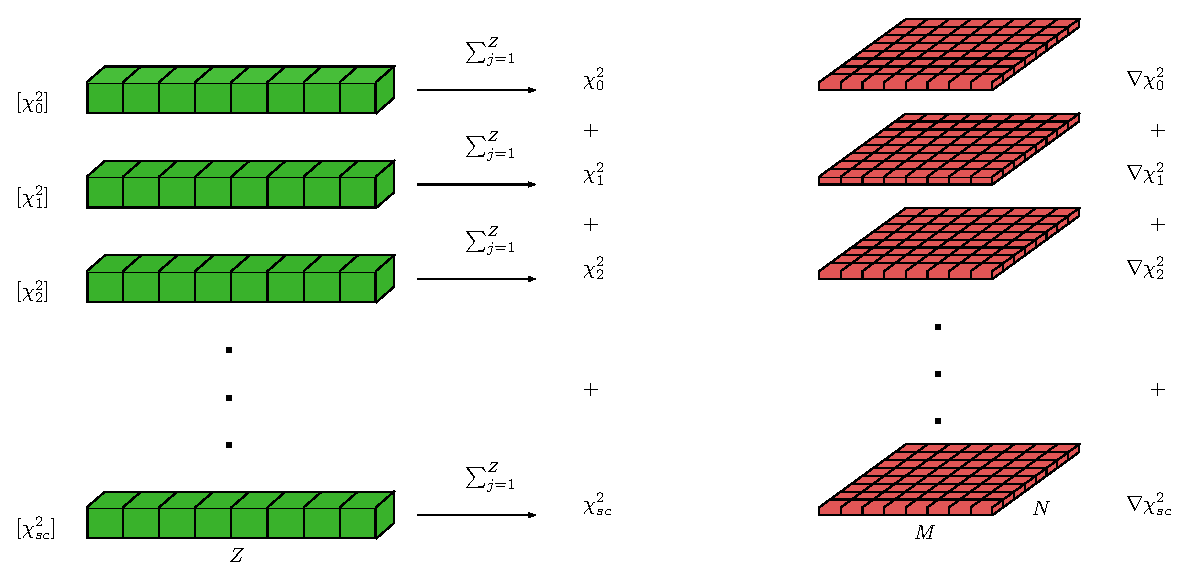
\includegraphics[scale=0.75]{./images/matrixandvector.eps}
    \caption{Ilustración del cálculo de $\chi^{2}$ y $\nabla \chi^{2}$ con conjuntos de datos multi-frecuencia. Fuente: Elaboración propia}
    \label{fig:matrixandvector}
\end{figure}





\chapter{Optimización}
\label{cap:opti}

En este capítulo se aborda el uso de método de gradiente conjugado para la minimización de la función no lineal \ref{eq:phiFinal}, destacando su funcionamiento y como esto se aplica a el problema abordado.

\section{Métodos de gradiente conjugado en múltiples dimensiones}

Los dos métodos de gradiente conjugado más importantes son el método de Fletcher-Reeves y el método de Polak-Ribiere. Estos métodos están relacionados puesto que sólo un paso de su algoritmo los diferencia. Estos algoritmos convergen al mínimo de una función en un número finito de iteraciones, para ello se localiza el intervalo donde se encuentra el mínimo, y luego se reduce.

\begin{algorithm}
\begin{algorithmic}[1]
    \STATE{Select $I_{0} \in \Re^{n}$}
    \STATE{$d_{0} = -\nabla \Phi(I_{0})$}
    \FOR{i=0 \TO MAX ITERATIONS}
        \STATE{Compute $\alpha_{i}$ such that $\Phi(I_{i}+\alpha_{i}d_{i}) = \min_{\alpha}\Phi(I_{i}+\alpha_{i}d_{i})$}
        \STATE {Set $I_{i+1} = I_{i}+ \alpha_{i}d_{i}$}
        \IF{$\left|\left|\nabla \Phi(I_{i+1})\right|\right| = 0$}
            \STATE{Stop.}
        \ELSE
            \STATE{$g_{i+1} = - \nabla \Phi(I_{i+1}) $}
            \STATE{$\beta_{i}=\frac{g_{i+1}^{T}g_{i+1}}{d_{i}^{T}d_{i}}$} \COMMENT{Fletcher-Reeves}
            \STATE{$\beta_{i}=\frac{g_{i+1}^{T}(g_{i+1}-d_{i})}{d_{i}^{T}d_{i}}$} \COMMENT{Polak-Ribiere}
            \STATE{$d_{i+1} = g_{i+1} + \beta_{i}d_{i}$}
        \ENDIF
    \ENDFOR
\end{algorithmic}
\caption{Algoritmo de Fletcher-Reeves/Polak-Ribiere}
\label{alg:polakribiere}
\end{algorithm}

En el algoritmo \ref{alg:polakribiere} las líneas 1 y 2 muestran que el algoritmo comienza con una imagen positiva plana y que luego se calcula la dirección de búsqueda inicial. En la línea 3 comienza el ciclo para encontrar el mínimo. Para calcular la siguiente imagen se debe encontrar un valor $\alpha$ que minimice la función objetivo siguiendo la dirección de búsqueda y sujeta a la restricción de positividad. En la línea 6, el algoritmo valida si se ha encontrado el mínimo, si se encuentra, entonces el algoritmo se detiene, de lo contrario se calcula un nueva dirección de búsqueda usando el valor de $\beta$ según Fletcher-Reeves (línea 10) o Polak-Ribiere (línea 11). Este último punto es importante, debido a que estas dos formas funcionan de la misma manera para ecuaciones de forma cuadrática. Sin embargo, en la realidad las funciones no son exactamente cuadráticas, y llegando al mínimo de la forma cuadrática se hace necesario llevar a cabo otro conjunto de iteraciones. En ese sentido, la fórmula de Polak-Ribiere funciona mejor cuando se hace necesario llegar hasta estos puntos \citep{numericalrecipes}.



\chapter{Multi-GPU}
\label{cap:multigpu}
La tarjeta Tesla K80 es una GPU que contiene dos tarjetas en una sola. Junto a ello, un sistema puede tener múltiples tarjetas GPU de alto cómputo. Por lo que se han querido aprovechar estas características para construir una solución que pueda ser usada tanto en una sola GPU como en múltiples, permitiendo así conseguir un mayor \textit{speedup}. A continuación se especifican las características de la solución para múltiples GPU.



\section{Comunicación Peer-to-Peer}
Una tarjeta puede comunicarse con la memoria de otra si es que la aplicación es ejecutada como un proceso de 64-bit y si la capacidad de cómputo de las tarjetas es 2.0 o más. Por ejemplo, una función que se ejecuta en GPU (\textit{kernel}) puede ejecutarse en una tarjeta y referenciar a un puntero cuya memoria haya sido almacenado en otra. Esto permite que la comunicación entre tarjetas sea más rápida debido a que si el acceso \textit{peer-to-peer} se habilita por medio de \texttt{cudaDeviceEnablePeerAccess()} ya no es necesario que los datos pasen por la memoria del sistema \citep{cuda}.
%Imagen Peer-to-Peer
Antes de utilizar la tecnología \textit{peer-to-peer} es necesario saber cuál es la topología del sistema para saber como los dispositivos PCI Express se conectan entre ellos y con CPU, esto es posible mediante el comando \texttt{nvidia-smi topo -m}. Por ejemplo, la topologia de Belka, sistema en donde se hacen las pruebas de este trabajo, puede verse en la Tabla \ref{tab:topology}.

\begin{table}[h!]
\centering
\begin{tabular}{@{}ccccccccc@{}}
\toprule
      & GPU 0 & GPU 1 & GPU 2 & GPU 3 & GPU 4 & GPU 5 & GPU 6 & GPU 7 \\ \midrule
GPU 0 & X     & PIX   & PHB   & PHB   & SOC   & SOC   & SOC   & SOC   \\
GPU 1 & PIX   & X     & PHB   & PHB   & SOC   & SOC   & SOC   & SOC   \\
GPU 2 & PHB   & PHB   & X     & PIX   & SOC   & SOC   & SOC   & SOC   \\
GPU 3 & PHB   & PHB   & PIX   & X     & SOC   & SOC   & SOC   & SOC   \\
GPU 4 & SOC   & SOC   & SOC   & SOC   & X     & PIX   & PHB   & PHB   \\
GPU 5 & SOC   & SOC   & SOC   & SOC   & PIX   & X     & PHB   & PHB   \\
GPU 6 & SOC   & SOC   & SOC   & SOC   & PHB   & PHB   & X     & PIX   \\
GPU 7 & SOC   & SOC   & SOC   & SOC   & PHB   & PHB   & PIX   & X     \\ \bottomrule
\end{tabular}
\caption{Topología de Belka}
\label{tab:topology}
\end{table}

Las sigla PIX representa una comunicación a través de switch PCI Express interno, PHB representa la comunicación a través de un \textit{host bridge} PCI Express y finalmente SOC representa la comunicación a nivel de socket. Esto nos dice que hay 4 Tesla K80 conectadas al sistema (recordar que una Tesla K80 contiene dos tarjetas conectadas mediante un switch interno) pero que un par está separado de otro mediante un socket. Por lo tanto, solo es posible realizar comunicación P2P entre las GPU cero, uno, dos y tres; y las GPU, cuatro, cinco, seis, y siete.

\section{Direccionamiento Virtual Unificado}

Es posible que todos los dispositivos GPU y la CPU, utilicen un único espacio de memoria si todos los dispositivos tienen una capacidad de cómputo mayor o igual a 2.0. Como consecuencia, cuando se copia memoria a un dispositivo que está usando un espacio de direcciones unificado el parámetro \texttt{cudaMemcpyKind} de \texttt{cudaMemcpy()}, puede ser seteado a \texttt{cudaMemcpyDefault} para que CUDA automáticamente determine donde se encuentra almacenada la memoria de los punteros \citep{cuda}.

Cualquier puntero de memoria en algún dispositivo puede ser creado por un \textit{thread} del host y puede ser directamente referenciado dentro del mismo proceso. Sin embargo, esto no es posible fuera del proceso, por lo tanto, no se puede referenciar directamente a un puntero de memoria que pertenezca a un proceso distinto. Es por ello que para paralelizar el uso de múltiples GPU, y debido a que los threads que se crean pertenecen al mismo proceso se ha optado por usar OpenMP \citep{cuda}.

\section{OpenMP}

Para acelerar el cálculo de $\chi^{2}$ y $\nabla \chi^{2}$ es necesario que el uso de las múltiples tarjetas sea de forma paralela. Para ello, hay que tener en cuenta que cualquier thread del proceso ejecutado puede ejecutar la instrucción \texttt{cudaSetDevice(x)} que cambia la GPU con la cual se trabajará, por lo que los \textit{kernels} que sean ejecutados desde ese punto en adelante serán ejecutados en la GPU $x$. Es posible usar esta instrucción de forma paralela y así hacer que cada thread invoque \textit{kernels} en una GPU distinta y de forma concurrente.


\chapter{Pruebas}
\label{cap:pruebas}

Para validar la solución se hace necesario enfocar las pruebas en dos aspectos del algoritmo implementado. Por un lado, se tienen las pruebas de aceleración, es decir, saber cuánto más rápido es MEM implementado en GPU, comparado con la solución \textit{multi-thread}. Por otra parte, se tienen las pruebas de caracterización que consisten en encontrar distintas características del algoritmo, tales como la resolución, nivel de ruido, entre otras.

A continuación, se presentarán con más detalle cada uno de estos aspectos.

\section{Benchmarks}
Según lo visto, el cálculo de $\Phi$ y $\nabla \Phi$ dependen tanto del número de visibilidades que se tengan en el set de datos como del número de píxeles de la imagen a reconstruir. Es por ello que para ver cuánto más rápido es el algoritmo es necesario escalar en ambas variables y comparar los resultados obtenidos con la solución multihebreada de MEM.

Además, de hacer esta comparación, se debe analizar la aceleración obtenida usando múltiples GPU. Para ello, se harán pruebas con un set de datos que contenga más de un canal y así comparar los speed-ups, tanto con la solución multi-hebra como con la solución implementada en GPU usando una única tarjeta.

\section{Caracterización de MEM}

\chapter{Resultados}
\label{cap:resultados}

\chapter{Conclusiones}
\label{cap:conclusiones}


% ### Bibliografía de la tesis ###
\bibliographystyle{apa-good}
\bibliography{bibliografia}
\addcontentsline{toc}{chapter}{Bibliografía} % Comando para agregar el índice a la Tabla de Contenido

% ### Optativo: Anexos de la tesis ###
\appendix
\addappheadtotoc							% Agregar Apéndice al índice. En caso de no poseer anexos, comentar
% ### Anexos ###
% !TEX root = ./../tesis-usach.tex
% !TEX program = xelatex
% !BIB program = bibtex
\chapter{Cálculo del gradiente de la función objetivo}
\label{apendice:dphi}
\begin{equation}
\Phi = \chi^2 + \lambda S
\end{equation}
con
\begin{eqnarray}
\chi^2 & = & \frac{1}{2}\sum^{Z}_{j=1}{\frac{|V^{m}_{j} - V_{j}^{o}|^{2}}{\sigma_j^{2}}} \\
S & = & \sum^{n}_{k=1}{I_{k}\log{(I_{k}/G)}}
\end{eqnarray}
con $0 \leq \lambda < \infty$.

Calculando el gradiente de la función $\Phi$, es decir, derivando parcialmente con respecto a $I_{k}$:

\begin{equation}
[\nabla\Phi]_k = \frac{\partial \Phi}{\partial I_{k}} = \frac{\partial}{\partial I_{k}} \chi^{2} + \lambda \frac{\partial}{\partial I_{k}}S
\label{eq:fina}
\end{equation}



Primero derivamos la derivada de $\chi^2$.
\begin{eqnarray}
\frac{\partial\chi^{2}}{\partial I_{k}} & = & \frac{\partial}{\partial I_{k}}\frac{1}{2}\sum\limits_{j}\frac{(V^{m}_{j} - V_{j}^{o})^{*}\cdot(V^{m}_{j} - V_{j}^{o})}{\sigma_{j}^{2}}\\
                                        & = & \frac{1}{2}\sum\limits_{j}\frac{1}{\sigma_{j}^{2}}\bigg(\frac{\partial
                                         V^{m*}_{j}}{\partial I_{k}}\Bigl( V_{j}^{m} - V_{j}^{o}\Bigr)+\frac{\partial V_{j}^{m}}{\partial I_{k}}\Bigl(V_{j}^{m}- V_{j}^{o}\Bigr)^{*}\biggr)
\end{eqnarray}

Note que $V_j^{o}$ es constante y por lo tanto su derivada respecto a $I_k$ es cero.
Donde la transformada de Fourier de la imagen ($I$) es igual a :

\begin{equation}
V_{j}^{m}=\sum^{n}_{k=1}I_{k}e^{-2\pi i<X_k,Z_j>}
\end{equation}

Donde $Z_j=(u_j,v_j)$, $X_k=(x_k,y_k)$, y el producto interno $<(a,b),(c,d)>=ac+bd$. Luego el conjugado es:

\begin{equation}
V_{j}^{m*}=\sum^{n}_{k=1}I_{k}e^{2\pi i<X_k,Z_j>}
\end{equation}

Derivando ambas visibilidades por separado con respecto a $I_{k}$ se tiene que:

\begin{eqnarray}
\frac{\partial V_{j}}{\partial I_{k}} & = & \exp\{-2\pi i<X_k,Z_j>\} \\
\frac{\partial V_{j}^{*}}{\partial I_{k}} & = & \exp\{+2\pi i<X_k,Z_j>\}
\end{eqnarray}

Definiedo el residuo de las visibilidades como:

\begin{equation}
V_{j}^{R} = V_{j}^{m}-V_{j}^{o} = \text{Re}(V_{j}^{R}) + i\cdot \text{Im}(V_{j}^{R})
\end{equation}

Y

\begin{equation}
V_{j}^{R*} = (V_{j}^{m}-V_{j}^{o})^{*}=\text{Re}(V_{j}^{R})-i\cdot \text{Im}(V_{j}^{R})
\end{equation}

Reemplazando estos términos se tiene:


\begin{equation}
\frac{\partial\chi^{2}}{\partial I_{k}} = \frac{1}{2}\sum\limits_{j}\frac{1}{\sigma_{j}^{2}}\Bigl[\exp\{2\pi i<X_k,Z_j>\}\Bigl(\text{Re}(V_{j}^{R})+i\text{Im}(V_{j}^{R})\Bigr)+
              \exp\{-2\pi i<X_k,Z_j>\}\Bigl(\text{Re}(V_{j}^{R})-i\text{Im}(V_{j}^{R})\Bigr)\Bigr]
\end{equation}

Multiplicando distributivamente:
%\begin{equation}
\begin{multline}
\frac{\partial\chi^{2}}{\partial I_{k}} = \frac{1}{2}\sum\limits_{j}\frac{1}{\sigma_{j}^{2}}\biggl[\exp\{2\pi i<X_k,Z_j>\}\text{Re}(V_{j}^{R})+i\exp\{2\pi i<X_k,Z_j>\}\text{Im}(V_{j}^{R})-\\
\exp\{-2\pi i \langle X_k,Z_j \rangle\}\text{Re}(V_{j}^{R})-i\exp\{-2\pi i\langle X_k,Z_j \rangle\}\text{Im}(V_{j}^{R})\biggr]
\end{multline}
%\end{equation}


Factorizando por la partes reales e imaginarias de $V_{j}^{R}$:

\begin{multline}
\frac{\partial\chi^{2}}{\partial I_{k}} = \frac{1}{2}\sum\limits_{j}\frac{1}{\sigma_{j}^{2}}\biggl[\text{Re}(V_{j}^{R})\Bigl(\exp\{2\pi i<X_k,Z_j>\}+\exp\{-2\pi i<X_k,Z_j>\}\Bigr)+ \\ i\text{Im}(V_{j}^{R})\Bigl(\exp\{2\pi i<X_k,Z_j>\}-\exp\{-2\pi i<X_k,Z_j>\}\Bigr)\biggr]
\end{multline}

Usando las propiedades trigonométricas del seno y coseno se tiene que:

\begin{eqnarray}
\frac{\partial\chi^{2}}{\partial I_{k}} & = & \frac{1}{2}\sum\limits_{j}\frac{1}{\sigma_{j}^{2}}\biggl[2\text{Re}(V_{j}^{R})\cos(2\pi <X_k,Z_j>)+2i^{2}\text{Im}(V_{j}^{R})\sin(2\pi \langle X_k,Z_j\rangle )\biggr] \\
                                      & = & \sum\limits_{j}\frac{1}{\sigma_{j}^{2}}\biggl[\text{Re}(V_{j}^{R}) \cos(2\pi\langle X_k,Z_j\rangle) - \text{Im}(V_{j}^{R})\sin(2\pi \langle X_k,Z_j\rangle)\biggr]
\end{eqnarray}

Definiendo

\begin{equation}
W_{j} = \frac{1}{\sigma_{j}^{2}}
\end{equation}

tenemos finalmente que

\begin{equation}
\frac{\partial\chi^{2}}{\partial I_{k}} = \sum\limits_{j}W_{j}\biggl[Re(V_{j}^{R})\cos\bigl(2\pi \langle X_k,Z_j\rangle\bigr)-\text{Im}(V_{j}^{R})\sin\bigl(2\pi \langle X_k,Z_j\rangle\bigr)\biggr]
\label{eq:dchi2}
\end{equation}

Continuando con $\frac{\partial}{\partial I_{k}}S$

\begin{equation}
\frac{\partial S}{\partial I_{k}} = \frac{\partial}{\partial I_{k}}\sum\limits_{k}I_{k}\log(I_{k}/G)
\end{equation}

Esto es igual a:


\begin{equation}
\frac{\partial S}{\partial I_{k}} = 1+\log(I_{k}/G)
\end{equation}


Por tanto la coordenada $k$ de $\nabla\Phi$:

\begin{multline}
[\nabla \Phi]_k = \sum\limits_{j}W_{j}\biggl[\text{Re}(V_{j}^{R})\cos\bigl(2\pi \langle X_k,Z_j \rangle\bigr)-\text{Im}(V_{j}^{R})\sin\bigl(2\pi \langle X_k,Z_j \rangle\bigr)\biggr] +
\lambda(1 + \log(I_{k}/G))
\label{eq:dphifinal}
\end{multline}


\end{document}
%\\end